%% LyX 2.4.0 created this file.  For more info, see https://www.lyx.org/.
%% Do not edit unless you really know what you are doing.
\documentclass[11pt,english]{article}
\usepackage{lmodern}
\renewcommand{\familydefault}{\rmdefault}
\usepackage[T1]{fontenc}
\usepackage[latin9]{luainputenc}
\usepackage{geometry}
\geometry{verbose,tmargin=1in,bmargin=1in,lmargin=1in,rmargin=1in}
\usepackage{babel}
\usepackage{amstext}
\usepackage{graphicx}
\usepackage{setspace}
\usepackage[authoryear]{natbib}
\onehalfspacing
\usepackage[pdfusetitle,
 bookmarks=true,bookmarksnumbered=false,bookmarksopen=false,
 breaklinks=false,pdfborder={0 0 0},pdfborderstyle={},backref=false,colorlinks=false]
 {hyperref}

\makeatletter

%%%%%%%%%%%%%%%%%%%%%%%%%%%%%% LyX specific LaTeX commands.
%% Because html converters don't know tabularnewline
\providecommand{\tabularnewline}{\\}

%%%%%%%%%%%%%%%%%%%%%%%%%%%%%% User specified LaTeX commands.
\date{}
% Added by lyx2lyx
\setlength{\parskip}{\medskipamount}
\setlength{\parindent}{0pt}

\ifdefined\showcaptionsetup
 % Caption package is used. Advise subfig not to load it again.
 \PassOptionsToPackage{caption=false}{subfig}
\fi
\usepackage{subfig}
\makeatother

\begin{document}
\title{Poverty Mapping in the Age of Machine Learning\thanks{The authors acknowledge financial support from the World Bank. We
thank Roy van der Weide and Isabel Molina for comments. Additionally,
we thank Benu Bidani, Carlos Rodriguez-Castelan, and Johan Mistiaen
for providing support and space to pursue this work. Finally, we thank
the Global Solutions Group on Data for Policy. Any error or omission
is the authors\textquoteright{} responsibility alone.}}
\author{Paul Corral,\thanks{The World Bank Group - Poverty and Equity Global Practice (pcorralrodas@worldbank.org)}
Heath Henderson,\thanks{Department of Economics and Finance, Drake University, United States
of America} and Sandra Segovia\thanks{The World Bank Group - Poverty and Equity Global Practice}}
\maketitle
\begin{abstract}
Recent years have witnessed considerable methodological advances in
poverty mapping, much of which has focused on the application of modern
machine-learning approaches to remotely-sensed data. Poverty maps
produced with these methods generally share a common validation procedure,
which assesses model performance by comparing sub-national poverty
estimates with survey-based, direct estimates. While unbiased, direct
estimates can be imprecise measures of true poverty rates, meaning
that it is unclear whether these validation procedures are informative
of actual model performance. In this paper, we use a rich dataset
from Mexico to provide a more rigorous assessment of the modern approach
to poverty mapping by evaluating its performance against a credible
ground truth. We find that the modern method under-performs relative
to benchmark traditional methods, largely because of the limited predictive
capacity of remotely-sensed covariates. For a given covariate set,
we also find that machine learning produces more biased poverty estimates
than the traditional procedures, particularly for the poorest geographic
areas.

\vfill{}
\end{abstract}
\textbf{Key words:} Small-area estimation; poverty mapping; machine
learning; satellite imagery

\textbf{JEL classification: }C13; C55; C87; C15\pagebreak{}

\section{Introduction}

Poverty maps provide granular estimates of poverty at the sub-national
level in order to better inform the targeting of resources and support
the design of interventions tailored to local needs (\citealt{bedi2007more,elbers2007poverty}).
As household surveys are generally unrepresentative for small geographical
areas, producing detailed poverty maps typically requires using small-area
estimation, which consists of using statistical methods to predict
poverty levels on the basis of household- or area-level characteristics.
The basic procedure entails two steps: (1) using household survey
data, fit a statistical model of some welfare measure (e.g., poverty,
income, or wealth) to household- or area-level characteristics, and
(2) apply the model to data available for all households or geographical
units to estimate poverty at the sub-national level. At a minimum,
the procedure then requires a household survey and data that covers
all geographic areas to produce a sufficiently detailed map.

The literature on small-area estimation is rich and several variations
on this basic procedure have been proposed. Unit-level models generally
use survey and census data to conduct estimation and prediction at
the household level, assuming a parametric relationship between the
welfare measure and covariates \citep{hentschel1998combining,elbers2003micro,molina2010small}.
Unit-level models are not well-suited to situations where the survey
and census correspond to different years, which is often the case
in developing countries where censuses are conducted infrequently.
Area-level models are the leading parametric alternative for off-census
years and only use aggregate data on the geographical units of interest
for estimation and prediction \citep{fay1979estimates,torabi2014small}.
Unit-context models have also been suggested for off-census years
and are characterized by an estimation stage wherein household-level
measures are modeled as a parametric function of area-level characteristics
\citep{nguyen2012method,lange2018small,masaki2020small}.

Recent developments in poverty mapping have focused on the application
of machine learning to remotely-sensed data, largely in response to
the issue of out-of-date census information. These approaches also
use survey-derived welfare measures, but are distinguished by a first
stage where a machine-learning model is fit to remotely-sensed covariates
(e.g., data derived from satellite imagery or call detail records)
rather than census-based covariates. For example, \citet{chi2022microestimates}
matched data from several remotely-sensed data sources to survey-based
measures of ``village'' wealth for 56 countries, and then fit a
prediction model using gradient boosting machines.\footnote{Their remotely-sensed data includes high-resolution satellite imagery,
mobile phone data, topographic maps, and connectivity data from Facebook.} They then applied the model to the populated surface of 135 low-
and middle-income countries to develop granular poverty maps for each
country. Similar approaches have been used for individual countries,
including Rwanda \citep{blumenstock2015predicting}, Bangladesh \citep{steele2017mapping},
Belize \citep{hersh2021open}, and Sri Lanka \citep{engstrom2022poverty},
among others.\footnote{See \citet{jean2016combining}, \citet{pokhriyal2017combining}, \citet{yeh2020using},
\citet{lee2020high}, \citet{aiken2022machine} and \citet{newhouse2022small}
for examples of other recent applications.}

This alternative method -- which we refer to as the ``modern''
approach to poverty mapping -- consists of several practices that
differ from more traditional approaches. Most obviously, the modern
approach substitutes non-parametric statistical methods for the parametric
approaches traditionally used for poverty mapping. In addition, the
modern approach relies heavily on remotely-sensed covariates rather
than covariates derived from census or administrative data.\footnote{Traditional area-level models occasionally use remotely-sensed data.
See \citet{seitz2019they} for an application using publicly-available
geospatial data.} Further, maps produced with machine-learning methods generally share
a common validation procedure. The key feature of this procedure is
that model performance is assessed by calculating the $R^{2}$ from
a regression of the observed poverty measures on the estimates for
the same geographical units.\footnote{For examples of the above procedure, see \citet{jean2016combining},
\citet{pokhriyal2017combining}, \citet{steele2017mapping}, \citet{lee2020high},
\citet{yeh2020using}, or \citet{chi2022microestimates}. Note that
a few studies use a similar procedure, but fit the machine-learning
model to household-level data and then aggregate the model's predictions
to the geographic unit of interest \citep{blumenstock2015predicting,hersh2021open,aiken2022machine}.} There are several limitations to this procedure, but the most critical
is that it typically uses direct, sample-based estimates rather than
true poverty measures as a performance benchmark. While direct estimates
are unbiased, they can be imprecise estimates of the true measures,
meaning that it is unclear whether the validation procedure is informative
of actual model performance (see Section \ref{sec:validation}).

In this paper, we provide a more rigorous assessment of the performance
of the modern approach to poverty mapping. Our approach consists of
constructing a pseudo-census (hereafter ``census'') that we use
to conduct several simulation experiments. Our experiments entail
repeatedly drawing survey samples from the census where each sample
produces direct poverty estimates for the sampled geographic areas.
With each sample we obtain small-area estimates using traditional
and modern mapping methods. The presence of the census means that
we observe the ``true'' poverty measure corresponding to the direct
estimate. We use these true poverty measures to gain insight into
the performance of machine-learning methods when validated against
a credible ground truth. As population censuses rarely collect detailed
data on income or expenditures, we construct our census from a large-scale
survey conducted in Mexico: the Mexican Intercensal Survey of 2015. 

The results of our simulations can be summarized as follows. First,
we find that poverty maps produced using machine learning and remotely-sensed
covariates tend to perform poorly relative to the traditional approach,
both in terms of the mean squared error of the estimates and simulated
targeting performance. Second, we find that this under-performance
is due to the low predictive capacity of the remotely-sensed covariates.
Machine learning performs comparably to, and sometimes better than,
the traditional methods when both methods use the same covariates.
Third, we show that the performance advantage of machine learning
for a given covariate set results from the relatively low variance
of its estimates, but this variance reduction comes at the cost of
increasing the bias of the estimates, particularly for the poorest
areas. This bias-variance trade-off is especially stark when using
remotely-sensed covariates and ultimately raises practical questions
about the use and production of modern poverty maps.

Our paper builds on the work of \citet{corral2021map} and \citet{corral2022guidelines},
who similarly used the Mexican Intercensal Survey to examine the performance
of several mapping methods. \citet{corral2021map} focused exclusively
on traditional mapping approaches and did not consider the performance
of machine-learning methods. While \citet{corral2022guidelines} consider
the performance of machine learning, their implementation only uses
census-based covariates and thus does not examine the performance
of the standard implementation that relies on remotely-sensed covariates.
Importantly, we are not the first paper to evaluate machine-learning
methods relative to independent census data. While \citet{yeh2020using}
and \citet{chi2022microestimates} validate their models relative
to a census, they focus on wealth rather than poverty and do not address
all the limitations of $R^{2}$ as a performance metric (see Section
\ref{sec:validation}). Finally, \citet{vanderweide2022how} examine
the performance of machine-learning methods combined with remotely-sensed
data, but not relative to true poverty measures.

This paper then represents the first attempt to rigorously assess
the performance of modern poverty-mapping methods relative to a ground
truth. The scope of our analysis is nevertheless limited in some important
ways. For one, we confine our attention to the performance of machine
learning for predicting income poverty and do not consider other welfare
measures, such as wealth or multi-dimensional poverty. We also focus
exclusively on the case of Mexico because of the unique data requirements
of our experiments and therefore do not assess the external validity
of our findings. A final limitation of our analysis is that we do
not consider all possible uses of machine learning for poverty mapping.
For example, we do not consider the issue of ``feature extraction,''
which is a data-processing technique that builds the covariates for
mapping exercises by applying machine learning to unstructured input
data (e.g., satellite imagery).\footnote{\citet{smythe2022geographic}, for example, used a convolutional neural
network to extract features from high-resolution satellite imagery
in Nigeria and then used those features to create a poverty map using
gradient boosting. See \citet{jean2016combining} or \citet{chi2022microestimates}
for other applications of a similar procedure.}

In what follows, Section \ref{sec:methods} discusses the various
methods we examine, including machine-learning methods and the traditional
approaches we use as performance benchmarks. Section \ref{sec:validation}
considers the issue of model validation by presenting a critical evaluation
of $R^{2}$ as a validation metric and proposing some alternative
measures. Section \ref{sec:data} then discusses the data we use for
our simulation experiments and Section \ref{sec:results} presents
the results. Finally, Section \ref{sec:conclusion} provides concluding
remarks, including practical recommendations for the production and
use of poverty maps.

\section{Methods\protect\label{sec:methods}}

This section describes the methods we use in our poverty-mapping simulations.
The first subsection discusses machine learning, with a special focus
on gradient boosting, as it is among the most popular machine-learning
methods for poverty mapping. The second subsection then discusses
more traditional approaches to poverty mapping, which we use as the
benchmark in our performance assessment of the machine-learning methods.

\subsection{Machine learning}

The goal of machine learning is to develop high-performance algorithms
for prediction, classification, and clustering/grouping tasks \citep{varian2014big,athey2018impact,athey2019machine}.
Such tasks can be divided into supervised and unsupervised learning
problems. While unsupervised learning focuses on identifying clusters
of observations that are similar in terms of their features, supervised
learning uses a set of features to predict some outcome of interest.
Supervised learning can be further divided into regression and classification
tasks, where regression is concerned with predicting continuous outcomes
and classification focuses on categorical outcomes. While there are
many machine-learning methods used for regression and classification
tasks (e.g., lasso, random forests, or support vector machines), the
following presents some key ideas by focusing on one of the leading
methods: gradient boosting.

Originally developed by \citet{friedman2001greedy}, gradient boosting
machines are a family of machine-learning techniques that combine
a large number of weak learners to form a stronger ensemble prediction.
Unlike some common ensemble techniques (e.g., random forests) that
simply average models in the ensemble, gradient boosting adds models
to the ensemble sequentially by fitting new weak learners to the negative
gradient of the chosen loss function. With the classic squared-error
loss function, this amounts to sequentially fitting new models to
the current residuals of the ensemble.\footnote{See \citet{natekin2013gradient} for an accessible introduction to
gradient boosting.} Extreme gradient boosting (XGBoost) is a particularly popular implementation
of gradient boosting that uses classification and regression trees
as the base models or weak learners. The popularity of XGBoost is
due to the fact that it is fast, scalable, and has been shown to outperform
competing methods across a wide range of problems \citep{chen2016xgboost}.

Classification and regression trees are based on a sequential binary
splitting of the covariate space that serves to partition the data
into subsamples that are increasingly homogeneous in terms of the
outcome variable. A tree begins with a single root node that is split
into two child nodes according to some decision rule. A decision rule
pertains to a single explanatory variable and observations are assigned
to the child nodes depending on whether they meet some condition associated
with the explanatory variable.\footnote{For example, for a continuous explanatory variable, one determines
whether a given observation falls above or below some numeric cutoff.} The child nodes can be further split into new child nodes based on
different decision rules that involve other explanatory variables
and cutoff points. Any child node that is not further split is referred
to as a terminal node or leaf, and each leaf is associated with a
parameter that provides a prediction for the subsample associated
with that leaf. For any given observation, the ensemble prediction
used by XGBoost is the sum of that observation's predictions across
all trees in the ensemble. 

To fix ideas, let $y_{i}^{d}$ denote the outcome of interest (e.g.,
direct estimates of poverty rates) for observation or entity $i$,
and let $x_{i}$ denote a vector of explanatory variables. In line
with the above, the predicted value of the outcome $y_{i}^{p}$ is
given by the sum of predictions across the individual trees in the
ensemble:

\begin{equation}
y_{i}^{p}=\sum_{t}f_{t}(x_{i})
\end{equation}
where the trees are indexed by $t$ and $f_{t}(x_{i})$ gives the
prediction of a given tree as a function of $x_{i}$. To build the
trees used in the model, XGBoost greedily minimizes the following
regularized objective function:

\begin{equation}
\mathcal{L}=\sum_{i}l(y_{i}^{d},y_{i}^{p})+\sum_{t}r(f_{t})
\end{equation}
where $l(y_{i}^{d},y_{i}^{p})$ is the loss associated with the $i^{th}$
observation and $r(f_{t})$ is a regularization term that serves to
mitigate overfitting.\footnote{For an in-depth discussion and description of the XGBoost algorithm
refer to \citet{chen2016xgboost}. Note that the fact that XGBoost
is a greedy algorithm means that a global minimum is not guaranteed.} In our implementation, we use the classic squared-error loss such
that $l(y_{i}^{d},y_{i}^{p})=(y_{i}^{d}-y_{i}^{p})^{2}$. 

XGBoost uses the following specification of the regularization term: 

\begin{equation}
r(f_{t})=\gamma M_{t}+\frac{1}{2}\lambda\sum_{j}m_{tj}^{2}
\end{equation}
where $M_{t}$ is the total number of leaves in tree $t$, $m_{tj}$
is the prediction associated with the $j^{th}$ leaf in a given tree,
and $\gamma$ and $\lambda$ are hyperparameters that must be chosen
by the user. The regularization term serves to mitigate overfitting
by penalizing complicated trees and smoothing the predictions associated
with each tree. That is, the method relies on a large number of weak
learners and the regularization term helps control the complexity
of the learners. It is important to note that the above specification
of the regularization term is only one of many possible specifications,
though \citet{chen2016xgboost} claim that it is simpler than the
leading alternatives and easier to parallelize. Further note that
when the hyperparameters are set to zero, the objective function becomes
equivalent to that used in traditional gradient boosting.

XGBoost requires the specification of several hyperparameters that
must be chosen by the user, including the hyperparameters in the regularization
term, the maximum tree depth, and the number of trees in the ensemble.
There are two additional hyperparameters that can be used to further
prevent overfitting. First, one can use column or feature subsampling
where each tree in the ensemble is built based on a (uniformly) random
subset of all explanatory variables. This procedure can also speed
up the algorithm because it reduces the number of covariates that
must be searched across when creating new splits. Second, one can
use shrinkage by scaling the predictions associated with each tree
by a factor $\eta$, which is often called the learning rate. The
predicted value of the outcome at iteration $t$ is then given by
the sum of the previous prediction and the current prediction scaled
by the learning rate. Shrinkage reduces the influence of each tree
so that no individual tree has too much influence on the ensemble
prediction.

One possible approach to hyperparameter selection is to use a grid
search where the user (1) specifies the domain of the hyperparameters,
(2) applies the model to every combination of hyperparameters, and
(3) selects the hyperparameters that perform the best in terms of
some metric (e.g., mean squared prediction error in the validation
dataset). Grid search, however, is computationally inefficient because
hyperparameter proposals are uninformed by previous evaluations. We
instead use a Bayesian hyperparameter optimization procedure, which
sequentially updates a probability model that relates the hyperparameter
space to the performance metric and then uses the model to intelligently
explore the hyperparameter space \citep{bergstra2011algorithms}.
Specifically, our implementation of gradient boosting relies on the
open-source library XGBoost, which we combine with the Hyperopt library
that conducts Bayesian hyperparameter optimization using the tree-structured
Parzen estimator.

\subsection{Traditional methods}

We benchmark the performance of the machine-learning approach against
two traditional poverty-mapping methods: the unit-level and area-level
models. Regarding unit-level models, the well-known methods of \citet{elbers2003micro}
and \citet{molina2010small} are based on the nested error model originally
proposed by \citet{battese1988asa}. This model assumes that (transformed)
equivalized household income or consumption relates to a vector of
household-level covariates according to the following model:

\begin{equation}
w_{iv}=x_{iv}\theta+\mu_{i}+\xi_{iv}\label{eq:sae-1}
\end{equation}

where $w_{iv}$ denotes the transformed equivalized income of household
$v$ in location $i$, $x_{iv}$ represents a vector of household-specific
characteristics, $\theta$ is a vector of coefficients on the household
characteristics, $\mu_{i}$ is location-specific random effect such
that $\mu_{i}\sim N(0,\sigma_{\mu}^{2})$, and $\xi_{iv}$ is a household-level
error term such that $\xi_{iv}\sim N(0,\sigma_{\xi}^{2})$.

The parameters of the model are typically estimated via restricted
maximum likelihood or Henderson's Method III (\citealt{henderson1953estimation}).\footnote{Henderson's Method III is coupled with generalized least squares to
obtain the regression coefficients.} Once the model is estimated, the parameters are then used to repeatedly
generate income estimates for all households in a corresponding census
dataset. That is, the income level of each household is predicted
$K$ times using the model estimates as follows:

\begin{equation}
w_{ivk}^{*}=x_{iv}\hat{\theta}+\mu_{ik}^{*}+\xi_{ivk}^{*}
\end{equation}

where $k$ indexes replications and where $\mu_{ik}^{*}$ and $\xi_{ivk}^{*}$
are drawn from their assumed distributions.\footnote{See \citet{rodas2021pull} for a more detailed description.}
As a final step, the replicates can be used to calculate $K$ estimates
of the poverty rate for each geographic entity and these estimates
can then be averaged to arrive at a final prediction for each area.
Note that there are multiple versions of the unit-level model, distinguished
primarily through different treatments of $\mu_{ik}^{*}$ and $\xi_{ivk}^{*}$.
We use a particular version known as the ``census empirical best''
method, which is a variant of the ``empirical best'' method of \citet{molina2010small}.\footnote{As opposed to empirical best estimates, census empirical best estimates
do not include survey observations when calculating area-level poverty
rates. \citet{rodas2021pull} show that when the sample size is small
relative to the population, the difference between the two methods
is negligible. For additional discussion, see \citet{molina2019desagregacion}.}

The key assumption of the unit-level model is that the distribution
of the explanatory variables is similar between the survey used for
estimation and the census used for prediction. This assumption is
generally violated if the census is outdated -- which is often the
case in developing countries -- and in this event the application
of the unit-level model will lead to similarly outdated poverty maps
\citep{lange2018small}. Importantly, machine-learning approaches
to poverty mapping are commonly motivated by the fact that censuses
are outdated and are thus viewed as a way to produce timely poverty
maps in a data-constrained environment. Stated differently, given
the differing data requirements between the unit-level model and the
machine-learning approach, the two methods are not generally considered
to be direct competitors. The unit-level model nevertheless serves
as a useful performance benchmark, as it is often viewed as the ``gold
standard'' of poverty mapping.

One closely related alternative, known as the unit-context model,
was specifically developed for use in off-census years. Initially
proposed by \citet{nguyen2012method} and later implemented by \citet{masaki2020small},
these models are based on a simple modification of the unit-level
approach: rather than modeling household-level income as a function
of household-level characteristics, unit-context models instead use
only area-level covariates from the census.\footnote{The key difference between the application from \citet{nguyen2012method}
and that of \citet{masaki2020small}, is that the former relied on
the approach presented by \citep{elbers2003micro} and the latter
relied on the approach introduced by \citep{molina2010small}. } Specifically, the unit-context model replaces the survey-based covariates
$x_{iv}$ in Eq.\,(\ref{eq:sae-1}) with census aggregates $x_{i}$
and thus relaxes the assumption that the survey-based covariates match
the moments of those from the census. The unit-context model is then
a direct competitor to the machine-learning approach because both
apply to off-census years. Recent research, however, has shown that
the unit-context model often produces biased and noisy poverty estimates,
largely due to its inability to explain between-household variation
in income \citep{corral2022guidelines,corral2021map,10.1111/rssa.12913}.\footnote{\citet{10.1111/rssa.12913,corral2022guidelines} both elaborate on
how the method also yields biased estimates of area-level means due
to the method's inherent bias.}

Due to these performance issues, the World Bank guidelines instead
recommend using the area-level models in off-census years \citep{corral2022guidelines}.\footnote{An earlier version of this paper also presented results on how area-level
models outperform, in terms of bias and noise, unit-context models
\citet{corral2023poverty}. } First proposed by \citet{fay1979estimates}, area-level models conduct
estimation and prediction using data aggregated to the geographic
area of interest. The area-level model consists of two basic parts.
The first part of the model links the actual or true poverty rates
$y_{i}^{a}$ for the $i^{th}$ entity to a vector of area-level covariates
$x_{i}$ as follows:

\begin{equation}
y_{i}^{a}=x_{i}\beta+\varepsilon_{i}\label{eq:linking-1}
\end{equation}

where $\beta$ is a vector of parameters to be estimated and $\varepsilon_{i}$
represents random area-level effects that are assumed to be mean zero
with a constant variance $\sigma_{\varepsilon}^{2}$.\footnote{While we focus on the original formulation of the model, note that
several extensions have been proposed, particularly to accommodate
more complicated error structures (e.g., spatial correlation). See
Chapter 3 of \citet{corral2022guidelines} for discussion.} Since we lack information on the true poverty rates, this model cannot
be immediately fit.

Instead, direct estimates of poverty rates from survey data $y_{i}^{d}$
are used as the outcome variable. These estimates are nevertheless
subject to sampling error because they are based on the area-specific
sample data. The second part of the model thus assumes that the direct
estimates are centered around the true poverty rates as follows:

\begin{equation}
y_{i}^{d}=y_{i}^{a}+\omega_{i}\label{eq:2nd=000020stage-1}
\end{equation}

where $\omega_{i}$ represents measurement or sampling error and is
assumed to have heteroskedastic variance $\sigma_{\omega,i}^{2}$
because sample sizes across areas are often unequal. These variances
are assumed to be known, although in practice they are estimated using
the survey data. Given the two parts of the model, the survey data
can then be used to obtain parameter estimates.

The best linear unbiased predictor (BLUP) is obtained by predicting
poverty rates through the model $x_{i}\hat{\beta}+\hat{\varepsilon}_{i}$
where $\hat{\beta}$ and $\hat{\varepsilon}_{i}$ represent the estimated
coefficients and area-level effects, respectively. More specifically,
the estimated area effect is $\hat{\varepsilon}_{i}=\psi_{i}\left(y_{i}^{d}-x_{i}\hat{\beta}\right)$
where $\psi_{i}=\hat{\sigma}_{\varepsilon}^{2}/\left(\hat{\sigma}_{\varepsilon}^{2}+\hat{\sigma}_{\omega,i}^{2}\right)$.
In essence, the final estimates for areas contained in the survey
are the weighted average between the direct estimate $y_{i}^{d}$
and the synthetic estimator $x_{i}\hat{\beta}$ where the weights,
$\psi_{i}$ and $(1-\psi_{i})$, are determined by the quality of
the model and the sample sizes for each area. For the non-sampled
entities, the area-level model simply uses the synthetic estimator
to produce predictions. A critical feature of the area-level model
is that it is a direct competitor to the machine-learning approach
because both methods are intended for use in off-census years and
do not rely on household-level data.

In summary, we use both the unit-level and area-level models as benchmarks
in our assessment of the modern approach to poverty mapping. While
the ``gold standard'' unit-level model provides an absolute performance
benchmark by approximating the upper performance bound, the area-level
model provides a relative performance benchmark as the leading competitor
to the modern approach. In our implementations of these models, we
follow World Bank guidelines and remove any eligible covariate that
is weak or extraneous \citep{corral2022guidelines}. For example,
when fitting the area-level model on a given sample, we sequentially
remove insignificant covariates from the set of eligible variables,
beginning with the one with the highest p-value. We then then address
collinearity by removing any variable with a variance inflation factor
above five.\footnote{See Section 3.2 in \citet{corral2022guidelines} for additional discussion.
Variable selection for the unit-level model is slightly more complicated,
as the above procedure is preceded by a lasso regression. See Section
6.2 in \citet{corral2022guidelines} for details.} All covariates enter into this procedure linearly because identifying
transformations (e.g., quadratic or cubic terms) would substantially
complicate our sampling experiments.

\section{Model Validation\protect\label{sec:validation}}

The coefficient of determination or $R^{2}$ is the most commonly
used metric for validating poverty maps generated using machine-learning
methods.\footnote{See \citet{jean2016combining}, \citet{pokhriyal2017combining}, \citet{steele2017mapping},
\citet{lee2020high}, \citet{yeh2020using}, or \citet{chi2022microestimates}.} In this section, we first critically assess this validation approach
by discussing three ways in which the $R^{2}$ can be misleading in
terms of model assessment. We then motivate our simulation experiments
by proposing an alternative approach that remedies many of the limitations
of the standard procedure. Specifically, we propose (1) assessing
model performance relative to true poverty measures rather than direct
estimates, and (2) using mean squared error and targeting performance
as the principal validation metrics. Our objective is to present a
validation procedure that is appropriate for our purposes rather than
a general strategy that is feasible for all poverty-mapping exercises.\footnote{For example, our validation procedure requires a dataset that is sufficiently
large for repeated sampling and such data is unlikely to be available
in many contexts. }

Regarding our assessment of the standard procedure, let $y_{i}^{a}$
denote the actual or true poverty indicator for the $i^{th}$ geographical
entity. Further, let $y_{i}^{d}$ and $y_{i}^{p}$ denote the direct
estimate and model-based prediction of the poverty indicator, respectively.
The standard method for assessing the predictive performance of model-based
poverty estimates calculates the $R^{2}$ from a regression like the
following:

\begin{equation}
y_{i}^{d}=\alpha+\delta y_{i}^{p}+\zeta_{i}
\end{equation}
where $\alpha$ and $\delta$ are the regression coefficients and
$\zeta$ represents the error term.\footnote{Note that any regression of this form can only be estimated for the
sampled regions with direct estimates.} The $R^{2}$ for the above regression can be written as follows:

\begin{equation}
R_{d}^{2}=\frac{\sigma_{d}^{2}-\sigma_{\zeta}^{2}}{\sigma_{d}^{2}}\label{eq:r2direct}
\end{equation}
where $\sigma_{d}^{2}$ is the variance of the direct estimate and
$\sigma_{\zeta}^{2}$ is the variance of $\zeta$. $R_{d}^{2}$ conveys
information about how much of the variance of the direct estimate
is explained by the model-based prediction. 

While unbiased, direct estimates can be imprecise estimates of true
poverty indicators \citep{rodas2021pull}. Ideally, one would assess
the performance of model-based predictions on the basis of the true
poverty indicators themselves. That is, model-based predictions are
more appropriately assessed using the $R^{2}$ from the following
regression:

\begin{equation}
y_{i}^{a}=\alpha+\delta y_{i}^{p}+\upsilon_{i}
\end{equation}
where $\upsilon$ represents the error term. The $R^{2}$ for this
regression can written as

\begin{equation}
R_{a}^{2}=\frac{\sigma_{a}^{2}-\sigma_{\upsilon}^{2}}{\sigma_{a}^{2}}\label{eq:r2true}
\end{equation}
where $\sigma_{a}^{2}$ is the variance of the true poverty indicator
and $\sigma_{\upsilon}^{2}$ is the variance of $\upsilon$. We are
first interested in characterizing the bias of $R_{d}^{2}$ when it
is used to approximate $R_{a}^{2}$.

Let $y_{i}^{d}=y_{i}^{a}+\omega_{i}$ where $\omega$ is a mean-zero
error term with variance $\sigma_{\omega}^{2}$. That is, we view
this as a classical measurement error problem where the direct estimate
of the poverty indicator is a noisy estimate of the true poverty indicator.\footnote{The assumption of classical measurement error may be violated in practice.
For example, if poorer households are less likely to be sampled, the
measurement error will not be independent of the true poverty rates. } Note that the preceding equation implies that $\zeta_{i}=\upsilon_{i}+\omega_{i}$
and $\sigma_{\zeta}^{2}=\sigma_{\upsilon}^{2}+\sigma_{\omega}^{2}$.
Following \citet{majeske2010quantifying}, we then define the bias
as:
\begin{equation}
B=R_{a}^{2}-R_{d}^{2}\,.\label{eq:bias}
\end{equation}
Substituting Eqs.\,(\ref{eq:r2direct}) and (\ref{eq:r2true}) into
our expression for the bias, we have:

\begin{equation}
B=\frac{\sigma_{a}^{2}-\sigma_{\upsilon}^{2}}{\sigma_{a}^{2}}-\frac{\sigma_{d}^{2}-\sigma_{\upsilon}^{2}-\sigma_{\omega}^{2}}{\sigma_{d}^{2}}=\frac{\sigma_{\omega}^{2}(\sigma_{a}^{2}-\sigma_{\upsilon}^{2})}{\sigma_{d}^{2}\sigma_{a}^{2}}=\frac{\sigma_{\omega}^{2}}{\sigma_{d}^{2}}R_{a}^{2}\,.\label{eq:bias_res}
\end{equation}
Finally, we can substitute Eq.\,(\ref{eq:bias_res}) into Eq.\,(\ref{eq:bias})
and rearrange, which gives

\begin{equation}
R_{d}^{2}=R_{a}^{2}\left(\frac{\sigma_{d}^{2}-\sigma_{\omega}^{2}}{\sigma_{d}^{2}}\right)\label{eq:relationship}
\end{equation}
and establishes a basic relationship between $R_{d}^{2}$ and $R_{a}^{2}$.
See \citet{majeske2010quantifying} for additional mathematical details. 

In Eq.\,(\ref{eq:relationship}) above, we see that $R_{d}^{2}=R_{a}^{2}$
when $\sigma_{\omega}^{2}=0$ or, equivalently, when $y_{i}^{d}=y_{i}^{a}$
for all $i$. In the presence of measurement error or when $\sigma_{\omega}^{2}>0$,
we then see that $R_{d}^{2}$ will be biased downward and the magnitude
of the bias will be determined by the size of $(\sigma_{d}^{2}-\sigma_{\omega}^{2})/\sigma_{d}^{2}$.
Validation exercises based on $R_{d}^{2}$ will thus tend to mischaracterize
the performance of poverty maps, with the resulting estimates of $R^{2}$
being biased downward. One implication of this bias is that $R_{d}^{2}$
is context-dependent and will generally be influenced by the design
of the survey data (e.g., larger sample sizes will tend to reduce
measurement error, all else equal). In particular, a poorly performing
model applied to a low bias setting may yield an estimate of $R_{d}^{2}$
that is higher than an estimate of $R_{d}^{2}$ from a strong model
applied to a high bias setting. The presence of bias in the measures
of $R^{2}$ can thus reverse the rank ordering of models when comparisons
are made across contexts.\footnote{See \citet{yeh2020using}, \citet{chi2022microestimates}, or \citet{aiken2022machine}
for this type of cross-context comparison of $R^{2}$ values.}

There is a second form of bias in $R^{2}$ that can conversely lead
to overoptimistic conclusions regarding model validity. To illustrate
this, note that $R_{a}^{2}$ in Eq.\,(\ref{eq:r2true}) is mathematically
equivalent to the squared (Pearson) correlation coefficient between
$y_{i}^{a}$ and $y_{i}^{p}$. A well-known property of the correlation
coefficient is that it is invariant to any positive affine transformation
of its arguments, implying that the \textit{squared} correlation coefficient
is invariant to \textit{any} affine transformation \citep{gujarati2003basic}.\footnote{More specifically, the correlation coefficient is invariant to any
\textit{positive} affine transformation because it changes signs when
one of its arguments is scaled by some negative constant. The \textit{squared}
correlation coefficient is then invariant to any affine transformation.} We can thus write
\begin{equation}
R_{a}^{2}(y_{i}^{a},y_{i}^{p})=R_{a}^{2}(y_{i}^{a},q_{1}+q_{2}y_{i}^{p})\label{eq:shift}
\end{equation}
where $q_{1}$ and $q_{2}$ are some arbitrary constants. The implication
of the above is that the $R^{2}$ is insensitive to systematic bias
in the model-based poverty estimates. Consider some unbiased poverty
estimate $y_{i}^{u}$, meaning that $E(y_{i}^{u}-y_{i}^{a})=0.$ Now
consider another estimate $y_{i}^{b}$ that is identical to $y_{i}^{u}$
up to some locational shift, implying that $y_{i}^{b}=y_{i}^{u}+q$
and $E(y_{i}^{b}-y_{i}^{a})=q$. While $y_{i}^{b}$ is biased (i.e.,
it will systematically over- or under-estimate poverty), it will misleadingly
achieve an $R^{2}$ that is identical to $y_{i}^{u}$. 

A third issue related to $R^{2}$ as a performance metric is that
it is affected by the variance of the true poverty measures. To see
this, consider the following re-expression of $R_{a}^{2}$:
\begin{equation}
R_{a}^{2}=1-\frac{\frac{1}{N}\sum_{i}(y_{i}^{a}-\alpha-\delta y_{i}^{p})^{2}}{\frac{1}{N}\sum_{i}(y_{i}^{a}-\bar{{y}}^{a})^{2}}=1-\frac{\text{{MSE}}(y_{i}^{a},\alpha+\delta y_{i}^{p})}{\text{{Var}}(y_{i}^{a})}\label{eq:variance}
\end{equation}
where $N$ is the number of geographical entities. The above shows
that $R^{2}$ can be viewed as a normalized version of the mean squared
error with the variance of the true poverty indicator used as the
normalization factor. This approach to normalization produces an additional
source of context-dependence in $R^{2}$. Consider two models that
perform equally well in that they achieve the same mean squared error.
However, assume that one model is applied to a context where the variance
of $y_{i}^{a}$ is large and the other is applied to a low-variance
context. The above implies that the model applied to the high-variance
context will achieve a higher $R^{2}$, even though the performance
of the two models is arguably identical. 

The limitations of the standard procedure stem both from the $R^{2}$
metric itself and from applying the $R^{2}$ to direct poverty estimates
rather than true poverty indicators. Accordingly, we address these
limitations by making two modifications to the usual procedure. To
address the issue related to error in the reference measure, we assess
our poverty-mapping methods with data that allows us to use true poverty
indicators as the reference measure (see the next section for discussion).
We then address the remaining limitations by focusing on validation
metrics that are sensitive to systematic biases in the poverty estimates
and avoid the normalization issue. To be clear, one could alternatively
attempt to correct the $R^{2}$ for its biases, but any adjustments
would require approximations that could lessen the credibility of
our validation exercises.\footnote{For example, correcting the bias associated with the measurement error
issue would require estimating the variance of the measurement error.}

Regarding our validation metrics, the mean squared error is closely
related to the $R^{2}$, but sidesteps its most critical limitations.
The mean squared error is defined as follows:

\begin{equation}
\text{{MSE}}(y_{i}^{a},y_{i}^{p})=\frac{{1}}{N}\sum_{i}(y_{i}^{a}-y_{i}^{p})^{2}\label{eq:mse}
\end{equation}

and we immediately see that it provides a direct understanding of
the expected squared error of the estimates and thus avoids the normalization
issue. It is also sensitive to systematic biases in the predictions.
Reconsidering the biased and unbiased poverty estimates described
above (i.e., $y_{i}^{u}$ and $y_{i}^{b}$), we can write $\text{{MSE}}(y_{i}^{b},y_{i}^{a})=\text{{MSE}}(y_{i}^{u}+q,y_{i}^{a})=\text{{MSE}}(y_{i}^{u},y_{i}^{a})+q^{2}$.
Systematic biases in the estimates will then be appropriately penalized
by the mean squared error. Another advantage is that with multiple
estimates for each entity, one can calculate entity-specific mean
squared errors, which can be decomposed into parts associated with
the bias and variance of the estimates. Where $y_{ih}^{p}$ denotes
estimate $h=1,2,\ldots,H$ for the $i^{th}$ entity, we have
\begin{equation}
\text{{MSE}}_{i}=\frac{{1}}{H}\sum_{h}(y_{i}^{a}-y_{ih}^{p})^{2}=\frac{{1}}{H}\sum_{h}(y_{ih}^{p}-\bar{{y}}_{i}^{p})^{2}+(\bar{{y}}_{i}^{p}-y_{i}^{a})^{2}\label{eq:mseg}
\end{equation}
where the first term on the right-hand side of the above captures
the variance of the estimates for entity $i$ and the second term
captures the (squared) bias.\footnote{See \citet{hastie2009elements} for derivation and detailed discussion
of the bias-variance decomposition.}

While calculating the error of the poverty estimates is useful for
understanding the accuracy of poverty maps, the primary reason for
obtaining granular poverty estimates is to improve the targeting of
resources. As such, we complement the mean squared error with an alternative
performance metric that focuses on how different methodological choices
affect poverty alleviation through influencing the efficiency of targeting.
Similar to \citet{elbers2007poverty}, we simulate a hypothetical
poverty-alleviation program that distributes resources to households
according to a given poverty map and then calculates the amount of
poverty-reduction associated with the map.\footnote{See \citet{yeh2020using}, \citet{chi2022microestimates}, and \citet{aiken2022machine}
for examples of other studies that have conducted targeting simulations.} Though using targeting performance as a validation metric has direct
policy relevance, note that it can be insensitive to systematic biases
in the poverty estimates (e.g., rank-based targeting schemes do not
depend on the absolute level of the poverty estimates).

The procedure we use in our simulations is as follows:

\vspace{-25bp}

\begin{enumerate}
\begin{singlespace}
\item Using true household-level incomes, calculate the poverty headcount
and poverty gap for the country as a whole for some chosen poverty
line. Using the poverty gap measure, determine the budget required
to completely eradicate poverty. Calculate an individual-level transfer
amount by dividing the total budget by the number of people living
in poverty. 
\item Using a given poverty map, order geographic areas according to their
estimated poverty headcounts, from most to least poor. For the poorest
area, augment the true per capita income of all households by an amount
equal to the transfer (i.e., each household receives an amount equal
to the transfer times the number of household members). Continue this
distribution procedure for the second poorest area, the third poorest
area, and so on until there are not enough resources to cover all
households in a given area. For the marginal area, distribute the
remaining budget equally among individuals in that area. 
\item Using the post-transfer household incomes, calculate an updated poverty
headcount to assess the effects of the distribution scheme on poverty
alleviation.
\end{singlespace}
\item Repeat steps 2 and 3 for each of the poverty maps generated by the
alternative methods.
\end{enumerate}
\vspace{-5bp}
The benchmark poverty alleviation from this scheme corresponds to
the results of applying the above to the true poverty rankings.

\section{Data\protect\label{sec:data}}

Carried out by the Mexican National Institute of Statistics and Geography
(INEGI) in 2015, the Mexican Intercensal Survey is a unique dataset
that allows us to construct a ground truth for our validation exercises.
The sample consists of 5.9 million households and is representative
at the national, state (32 states), and municipality level (2,457
municipalities). It is also representative for localities with populations
of 50,000 or more inhabitants. The survey questionnaire gathered information
on household income, geographic location, household demographics,
and dwelling characteristics, among other things.\footnote{Income is defined as money received from work performed during the
course of the reference period by individuals aged 12 or older.} The size of the dataset is especially important, as it allows us
conduct simulation experiments with repeated samples that are sufficiently
large and diverse. We use these samples to estimate municipality-level
poverty maps with alternative methods and then assess the maps using
the full dataset as the ground truth.

Prior to sampling from the intercensus, we make three modifications
to the data. First, as a large number of households reported earning
no income, we randomly remove 90 percent of these households.\footnote{This is done to ensure some missing values are present in the data
used, but not as many as in the original data.} Second, to ensure that all municipalities are sufficiently large,
municipalities with less than 500 households are removed. Finally,
to ensure that all primary sampling units (PSUs) are also sufficiently
large for sampling purposes, we combine several neighboring PSUs such
that all include at least 300 households. Our final census dataset
consists of 3.9 million households in 1,865 municipalities and 16,297
PSUs. The resulting census is used to draw 500 survey samples that
serve as the basis for our simulation experiments (\citealp{tzavidis2018start}).
In what follows, we describe our approach to constructing these samples.

Our sampling procedure is intended to reflect standard design elements
used in many face-to-face household surveys conducted in the developing
world \citep{grosh1996manual}. Mexico's 32 states comprise the intended
domains of the sample and the indicator of interest is household income
per capita. For each sample, we seek to achieve a relative standard
error (RSE) of 7.5 percent for average household income in each state.\footnote{The desired precision of 7.5 percent is somewhat arbitrary, but corresponds
to precision targets in similar surveys and yields samples of reasonable
sizes.} We use a two-stage clustered design wherein PSUs or clusters are
selected within each domain and then a sample of 10 households is
selected within each cluster. Our decision to select 10 households
within each cluster is consistent with the design of other large-scale
household surveys conducted in developing countries \citep{grosh1996manual}.
Under simple random sampling, the minimum sample size required for
each state is as follows:

\begin{equation}
n_{s}=\left(\frac{\sigma_{s}}{\bar{{w}}_{s}\times\text{{RSE}}}\right)^{2}
\end{equation}

where $\bar{{w}_{s}}$ and $\sigma_{s}$ represent average household
income per capita and the standard deviation of per capita income
for state $s$, respectively.

The minimum sample size under simple random sampling must be adjusted
to account for the clustered design. The design effect due to clustering
is accounted for by estimating the intra-cluster correlation of per
capita income within each state. The correlation estimates can then
be used to adjust the above sample sizes for the clustered design
as follows:

\begin{equation}
n_{s}\times\Big[1+\rho_{s}\left(n_{sc}-1\right)\Big]
\end{equation}

where $n_{sc}$ denotes the number of households selected in cluster
$c$ within state $s$ (10 in this case) and $\rho_{s}$ is the intra-cluster
correlation of per capita income. Given the above, we can calculate
the number of clusters needed to achieve the minimum sample size for
each state and then multiply this number by 10 to find the final sample
size. Taking these sample size requirements as given, each of our
samples is then drawn in accordance with the two-stage design.

Specifically, the clusters within each state are selected with probability
proportional to size (without replacement) and the households within
each cluster are selected via simple random sampling. According to
this design, the inclusion probability for a given household is then
approximately:

\begin{equation}
\frac{\tilde{{n}}_{sc}N_{s}}{\tilde{{n}}_{s}}\times\frac{n_{sc}}{\tilde{{n}}_{sc}}
\end{equation}

where $\tilde{{n}}_{sc}$ is the total number of households in cluster
$c$ within state $s$, $N_{s}$ is the number of clusters selected
in state $s$, and $\tilde{{n}}_{s}$ is the total number of households
in state $s$.\footnote{The equation used to calculate inclusion probabilities assumes sampling
with replacement, but is used here as an approximation of inclusion
probabilities under proportional selection without replacement. This
should provide a reasonable approximation in this case since there
are a relatively large number of clusters present in the frame. The
design weight for each household is simply the inverse of the inclusion
probability. In a typical survey, the design weights would be further
adjusted for nonresponse and calibrated to known population characteristics.
However, since the sampling is only a simulation exercise, there is
no nonresponse and thus no nonresponse adjustment is required. Calibration
or post-stratification could be performed, but was not implemented
to simplify the process.} Table \ref{tab:desc_stats} presents select descriptive statistics
related to the full intercensus and the 500 samples. We set the poverty
line at the 25th percentile of the true income distribution and the
first two rows summarize the associated poverty rates at the municipality
and PSU levels for the full dataset. The remaining rows summarize
our samples and show that we draw 23,540 households per sample (2,354
PSUs), with an average number of municipalities per sample of roughly
992. The samples thus have an average of 2.37 PSUs per municipality.

\begin{table}
\begin{onehalfspace}
\begin{centering}
\begin{tabular}{lccccc}
\hline 
Variable & Mean & Std. Dev. & Min. & Max. & Obs.\tabularnewline
\hline 
Municipality poverty rate (full intercensus) & 0.30 & 0.19 & 0.02 & 0.96 & 1,865\tabularnewline
PSU poverty rate (full intercensus) & 0.23 & 0.20 & 0.00 & 1.00 & 16,297\tabularnewline
Observations per sample  & 23,540 & 0.00 & 23,540 & 23,540 & 500\tabularnewline
PSU per sample & 2,354 & 0.00 & 2,354 & 2,354 & 500\tabularnewline
Municipalities per sample & 992.04 & 11.95 & 951 & 1,020 & 500\tabularnewline
PSU-to-municipality ratio per sample & 2.37 & 0.03 & 2.31 & 2.48 & 500\tabularnewline
\hline 
\end{tabular}
\par\end{centering}
\end{onehalfspace}
\caption{Select descriptive statistics for the Mexican Intercensal Survey\protect\label{tab:desc_stats}}

\end{table}

In addition to the intercensus, INEGI has also released geo-referenced
data that is similar to the remotely-sensed covariates often used
in machine-learning applications. These geographic variables were
calculated by INEGI for the year 2015 (the same year as the intercensus)
and the municipality is the lowest administrative level for which
the covariates are available.\footnote{Technically speaking, the intercensus does not include identifiers
that provide information on geographic location below the municipality
level. We are thus only able to merge the intercensus and geo-referenced
data at the municipality level.} The geo-referenced data includes 105 indicators. Specifically, the
dataset includes information from 21 different dimensions and each
dimension is associated with five summary measures.\footnote{The 21 dimensions are as follows: enhanced vegetation index, normalized
difference vegetation index, normalized difference built-up index,
built-up index, simple ratio, atmospherically resistant vegetation
index, urban index, index of biological integrity, normalized difference
water index, modified normalized difference water index, new built-up
index, band ratio for built-up area, normalized built-up area index,
built-up area extraction index, normalized difference snow index,
visible atmospherically resistant index, soil-adjusted vegetation
index, optimized soil-adjusted vegetation index, normalized difference
moisture index, digital altitude model, and digital slope model.} For example, we summarize the atmospherically resistant vegetation
index for each municipality using the minimum, maximum, mean, sum,
and standard deviation of the index. The same procedure is applied
to all dimensions. The geo-referenced data has one major limitation,
which is that it does not include information on night-time lights,
which is a commonly-used covariate in machine-learning applications.\footnote{For examples, see \citet{jean2016combining}, \citet{lee2020high},
or \citet{chi2022microestimates}.} 

We thus augment the INEGI geo-referenced data with night-time lights
data produced by the Earth Observation Group (EOG). EOG uses the nightly
day/night band (DNB) low light imaging data gathered by the NASA/NOAA
Visible Infrared Imaging Radiometer Suite (VIIRS) \citep{elvidge2021annual}.
To match the other geo-referenced covariates, we use the night-time
lights data from 2015, which is available at 15 arc-second resolution
(roughly 500 meters at the equator) and then aggregated to the municipality
level. Also like the other geo-referenced data, we summarize night-time
lights within each municipality using the minimum, maximum, mean,
sum, and standard deviation. With these additions, we then have two
alternative sets of covariates that we use in our simulations: the
geo-referenced data (including night-time lights) and the standard
set of sociodemographic covariates from the intercensus.

\section{Results\protect\label{sec:results}}

Recall that our primary objective is to assess the performance of
the modern approach to poverty mapping by using the Mexican Intercensal
Survey as a ground truth. To this end, panel (a) in Figure \ref{fig:mse_targeting}
presents the mean squared error (MSE) for our closest approximation
to the standard implementation of the modern approach: gradient boosting
with remotely-sensed covariates (covariates labeled ``GIS''). We
benchmark the performance of this implementation against two traditional
mapping methods, namely the unit-level and area-level models. To approximate
how these traditional methods are commonly used, each model is implemented
with census-based covariates, albeit at different levels of analysis
(covariates labeled ``CEN''). Importantly, as our initial implementations
are intended to reflect current practice, the modern and traditional
approaches differ both in terms of their statistical method and the
covariates used. The remainder of this section will examine how these
differences contribute to performance disparities between the two
approaches. 

\begin{figure}
\begin{centering}
\subfloat[Mean squared error]{\begin{centering}
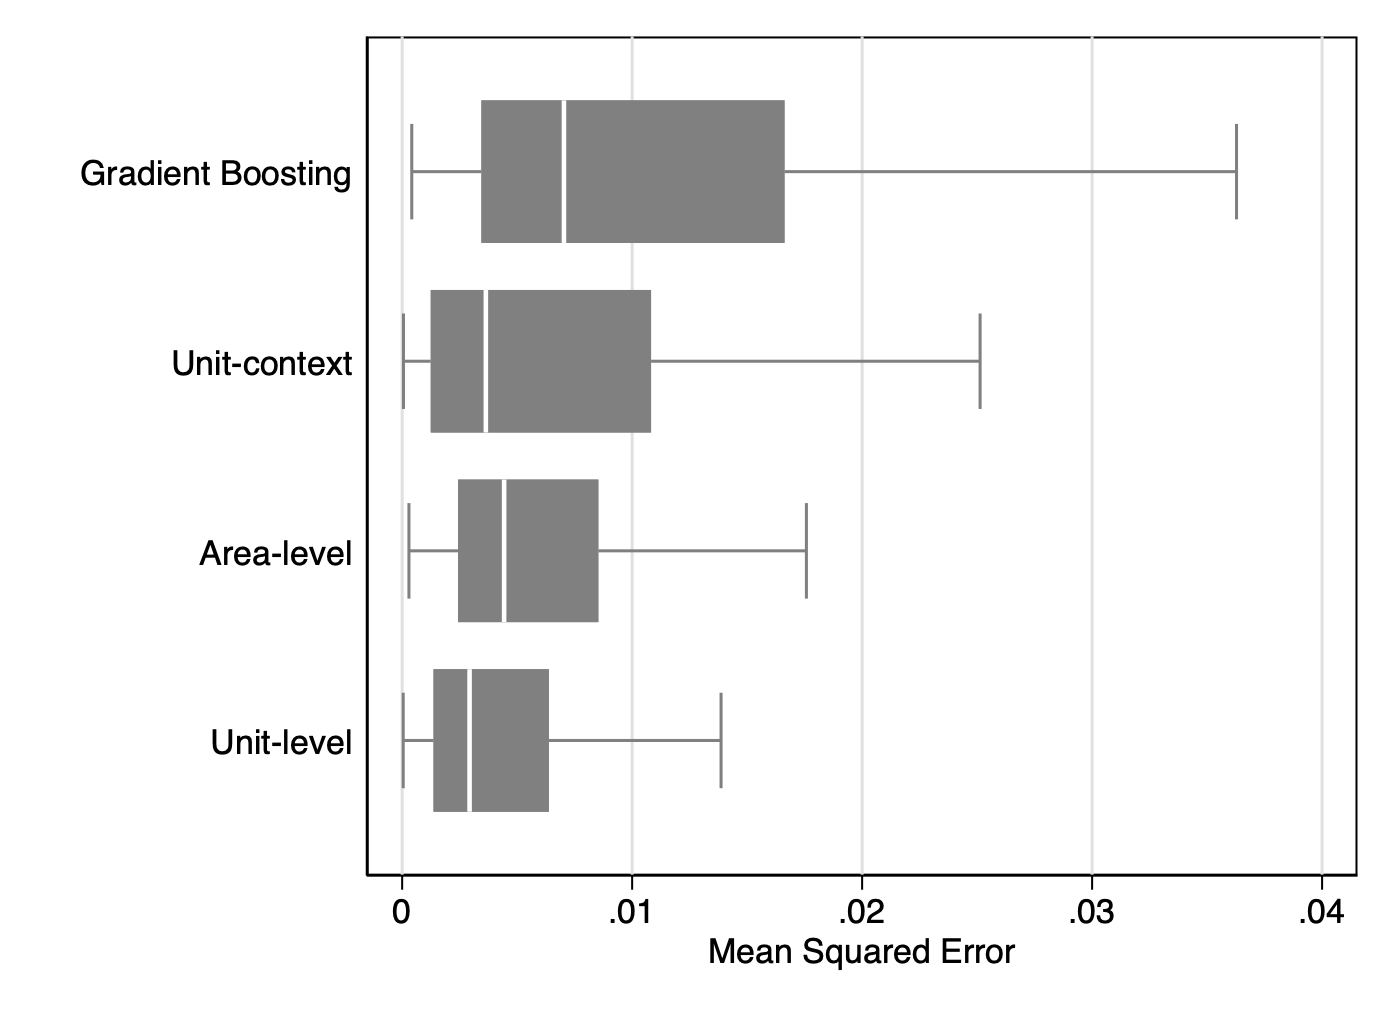
\includegraphics[scale=0.3]{Figure-1a}
\par\end{centering}
}\hspace{0cm}\subfloat[Targeting performance]{\begin{centering}
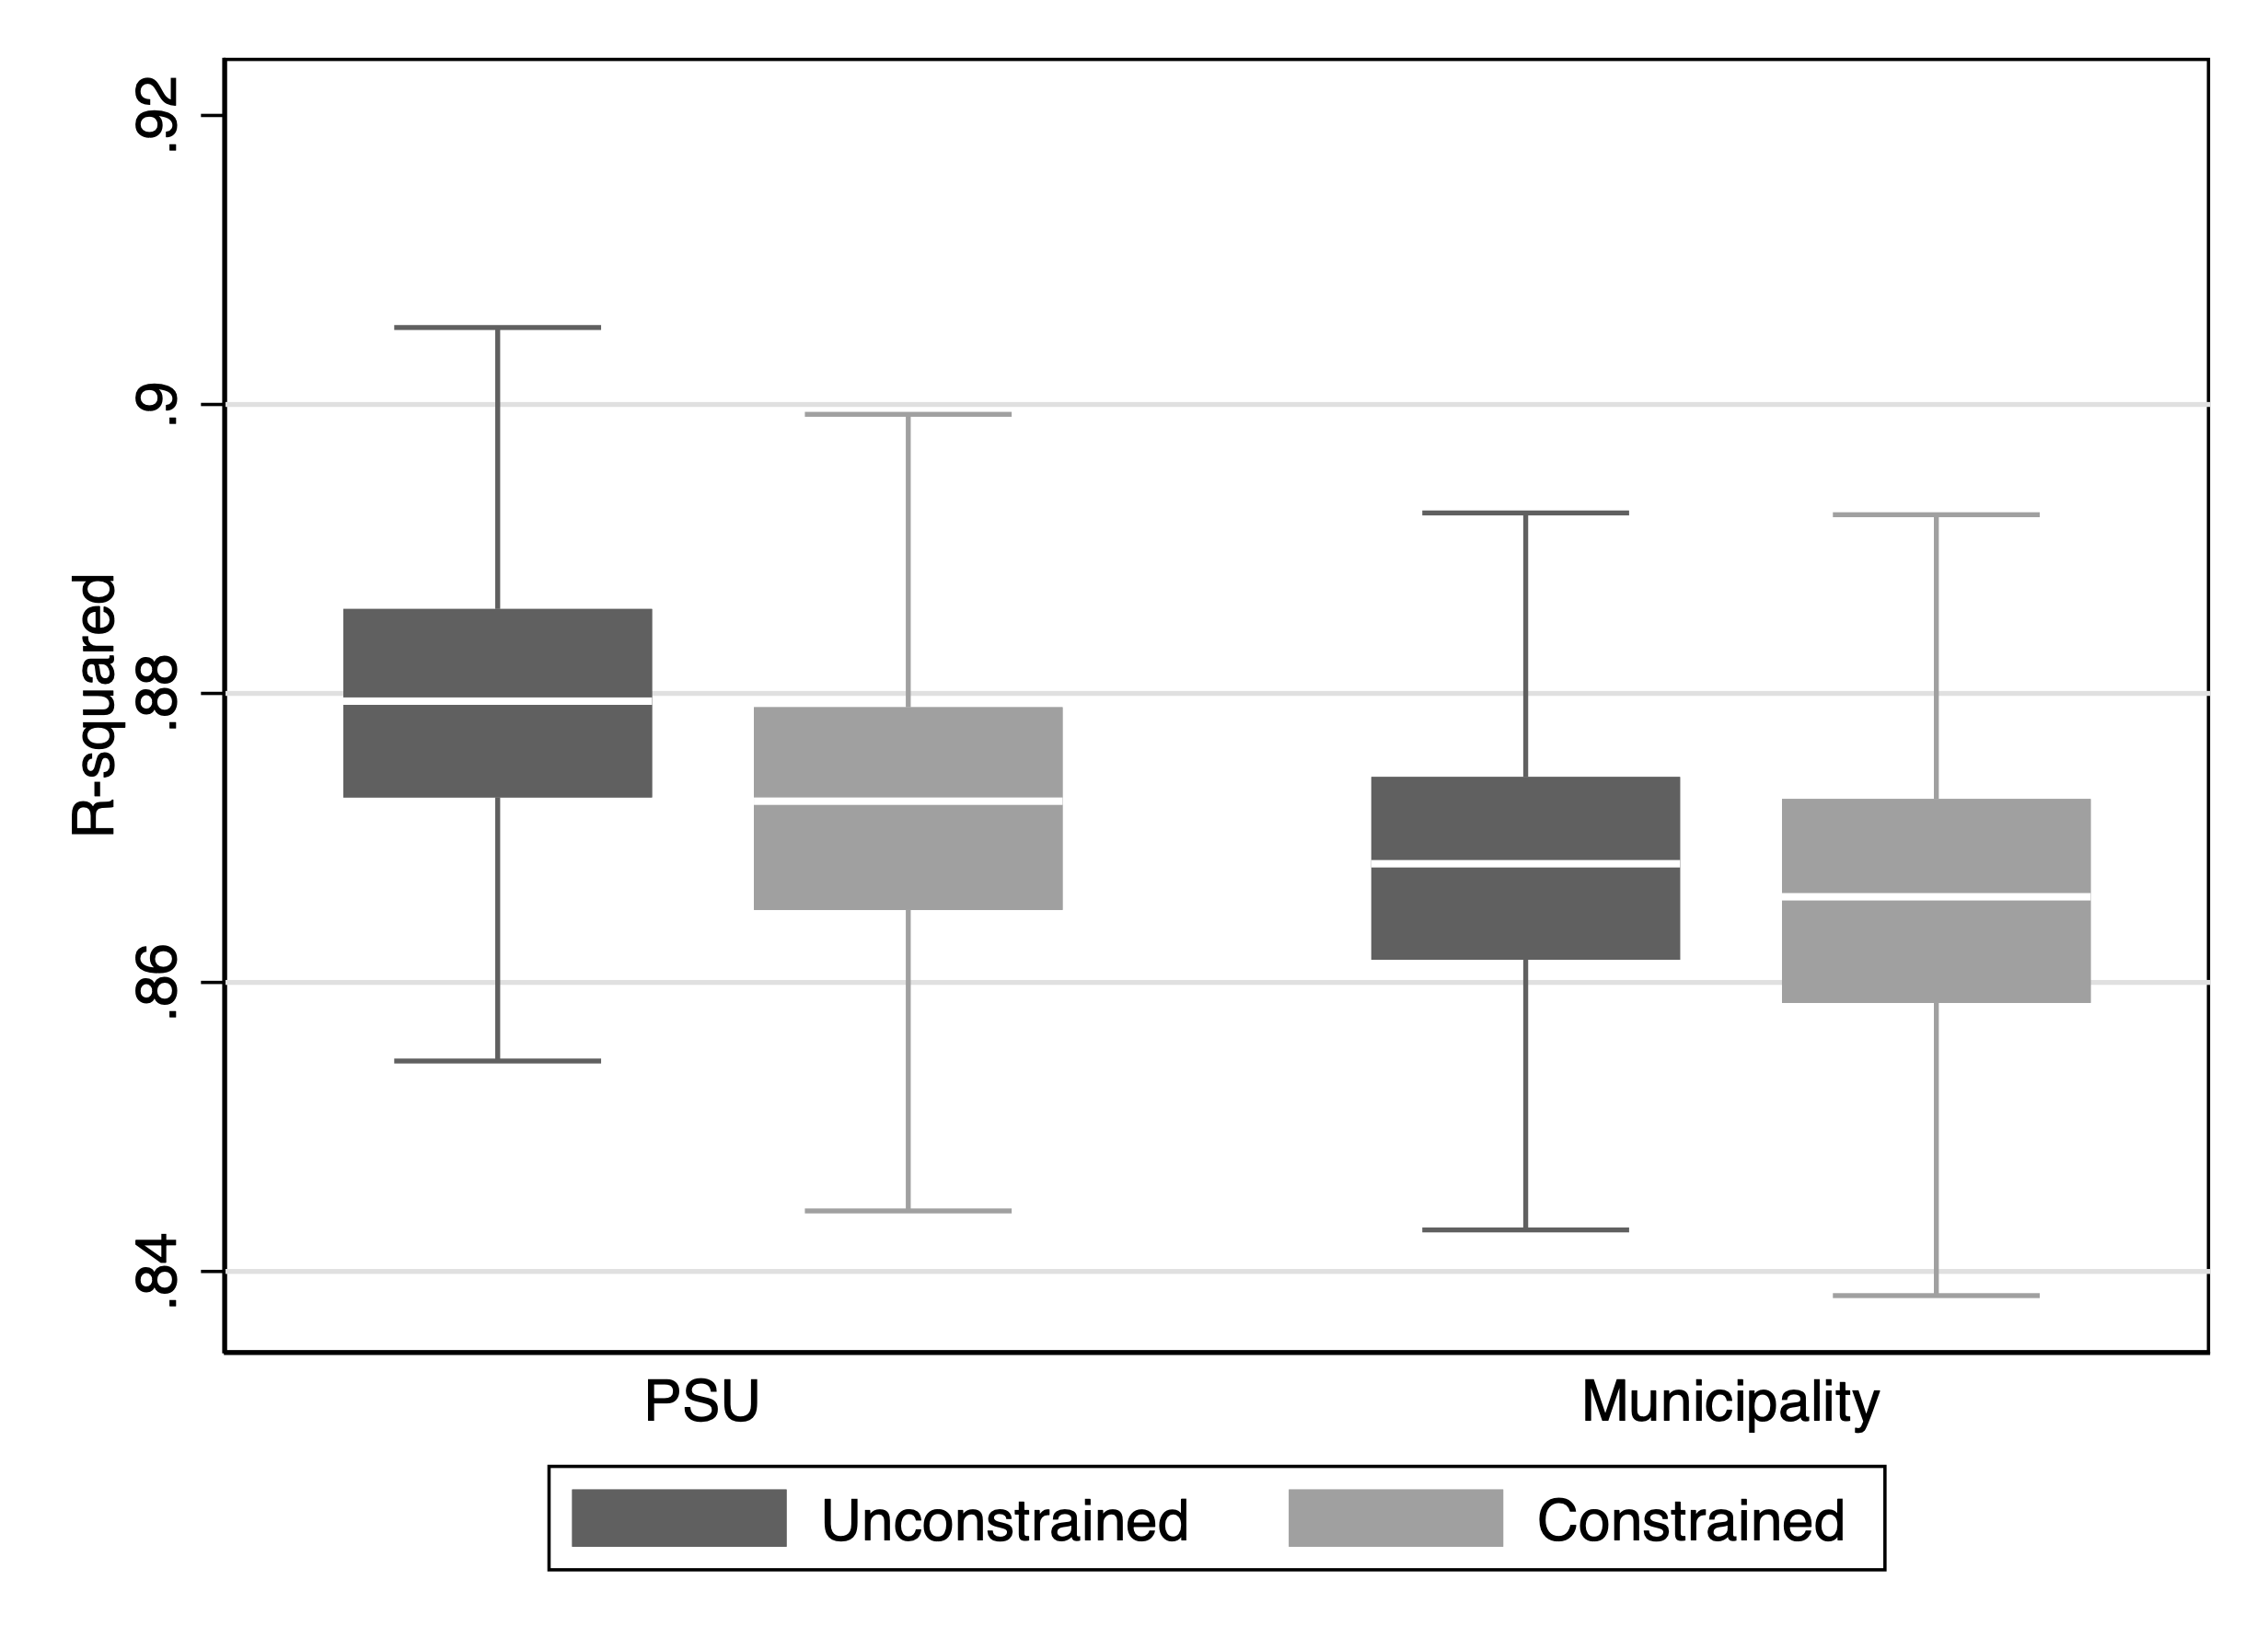
\includegraphics[scale=0.3]{Figure-1b}
\par\end{centering}
}
\par\end{centering}
\centering{}\caption{Mean squared error and targeting performance for select implementations
\protect\label{fig:mse_targeting}}
\end{figure}

Panel (a) of Figure \ref{fig:mse_targeting} shows that gradient boosting
with remotely-sensed covariates tends to have the highest MSE of the
models considered. The associated boxplot summarizes the distribution
of MSE values across all municipalities (i.e., the results are based
on Eq. {[}\ref{eq:mseg}{]}) and indicates that the gradient-boosting
model achieves a median MSE of 0.007. The corresponding root MSE is
approximately 0.08, meaning that the median municipality's error is
roughly eight percentage points. By contrast, the ``gold standard''
unit-level achieves a median MSE of 0.003, which is roughly 40 percent
that of the gradient-boosting model. The area-level model performs
similarly to the unit-level model, with a median MSE of 0.004. The
fact that the area-level model outperforms the gradient-boosting model
is particularly notable, as both of these models were developed for
use in off-census years and are thus direct competitors.

Panel (b) of Figure \ref{fig:mse_targeting} considers the targeting
performance of the alternative models and shows a similar result.
For these simulations, we have set the poverty line at the 25th percentile
of the (pre-transfer) per capita income distribution, which means
that the baseline poverty rate is 25 percent. The poverty rate falls
to 19.9 percent when transfers are delivered to municipalities according
to their true poverty rate. Across 500 simulations, we find that gradient
boosting with remotely-sensed covariates achieves a median poverty
rate of 20.29, which is close to the benchmark rate of 19.9 percent.
The two traditional methods nevertheless outperform the gradient-boosting
model. The unit-level model achieves a median poverty rate of 20 percent
whereas the area-level model achieves a median rate of 20.04. The
traditional approach thus outperforms the modern approach by about
0.3 percentage points, which in a country the size of Mexico corresponds
to about 360,000 additional people escaping poverty.\footnote{Mexico's population was about 120 million in 2015, which is the year
that the Mexican Intercensal Survey was conducted.}

As mentioned, there are two primary differences between the traditional
and modern approaches that could explain these performance disparities:
the statistical method and the covariates used. We first examine whether
using an alternative statistical method could improve upon the performance
of our initial implementation of the modern approach. Figure \ref{fig:alt_methods}
presents MSE and targeting results for four alternative statistical
methods where each uses the same, remotely-sensed covariates in order
to isolate the influence of the method. In addition to gradient boosting,
we consider two leading non-parametric competitors (i.e., random forest
and Bayesian additive regression trees) and the leading parametric
competitor (i.e., the area-level model).\footnote{In terms of non-parametric models, both random forests and Bayesian
additive regression trees are quite popular and have been shown to
perform comparably to, and sometimes better than, gradient boosting.
For example, see \citet{chipman2010bart}. } We find that the alternative methods do not produce any substantive
performance gains. In particular, the two alternative non-parametric
methods perform similarly to gradient boosting whereas the parametric,
area-level model tends to perform slightly worse when using the same
covariates.\footnote{Bayesian additive regression trees perform slightly better than gradient
boosting, but the performance gains are not large. For example, in
terms of targeting performance, gradient boosting achieves a median
poverty rate of 20.29 whereas the Bayesian method achieves a median
rate of 20.26. }

\begin{figure}
\begin{centering}
\subfloat[Mean squared error]{\begin{centering}
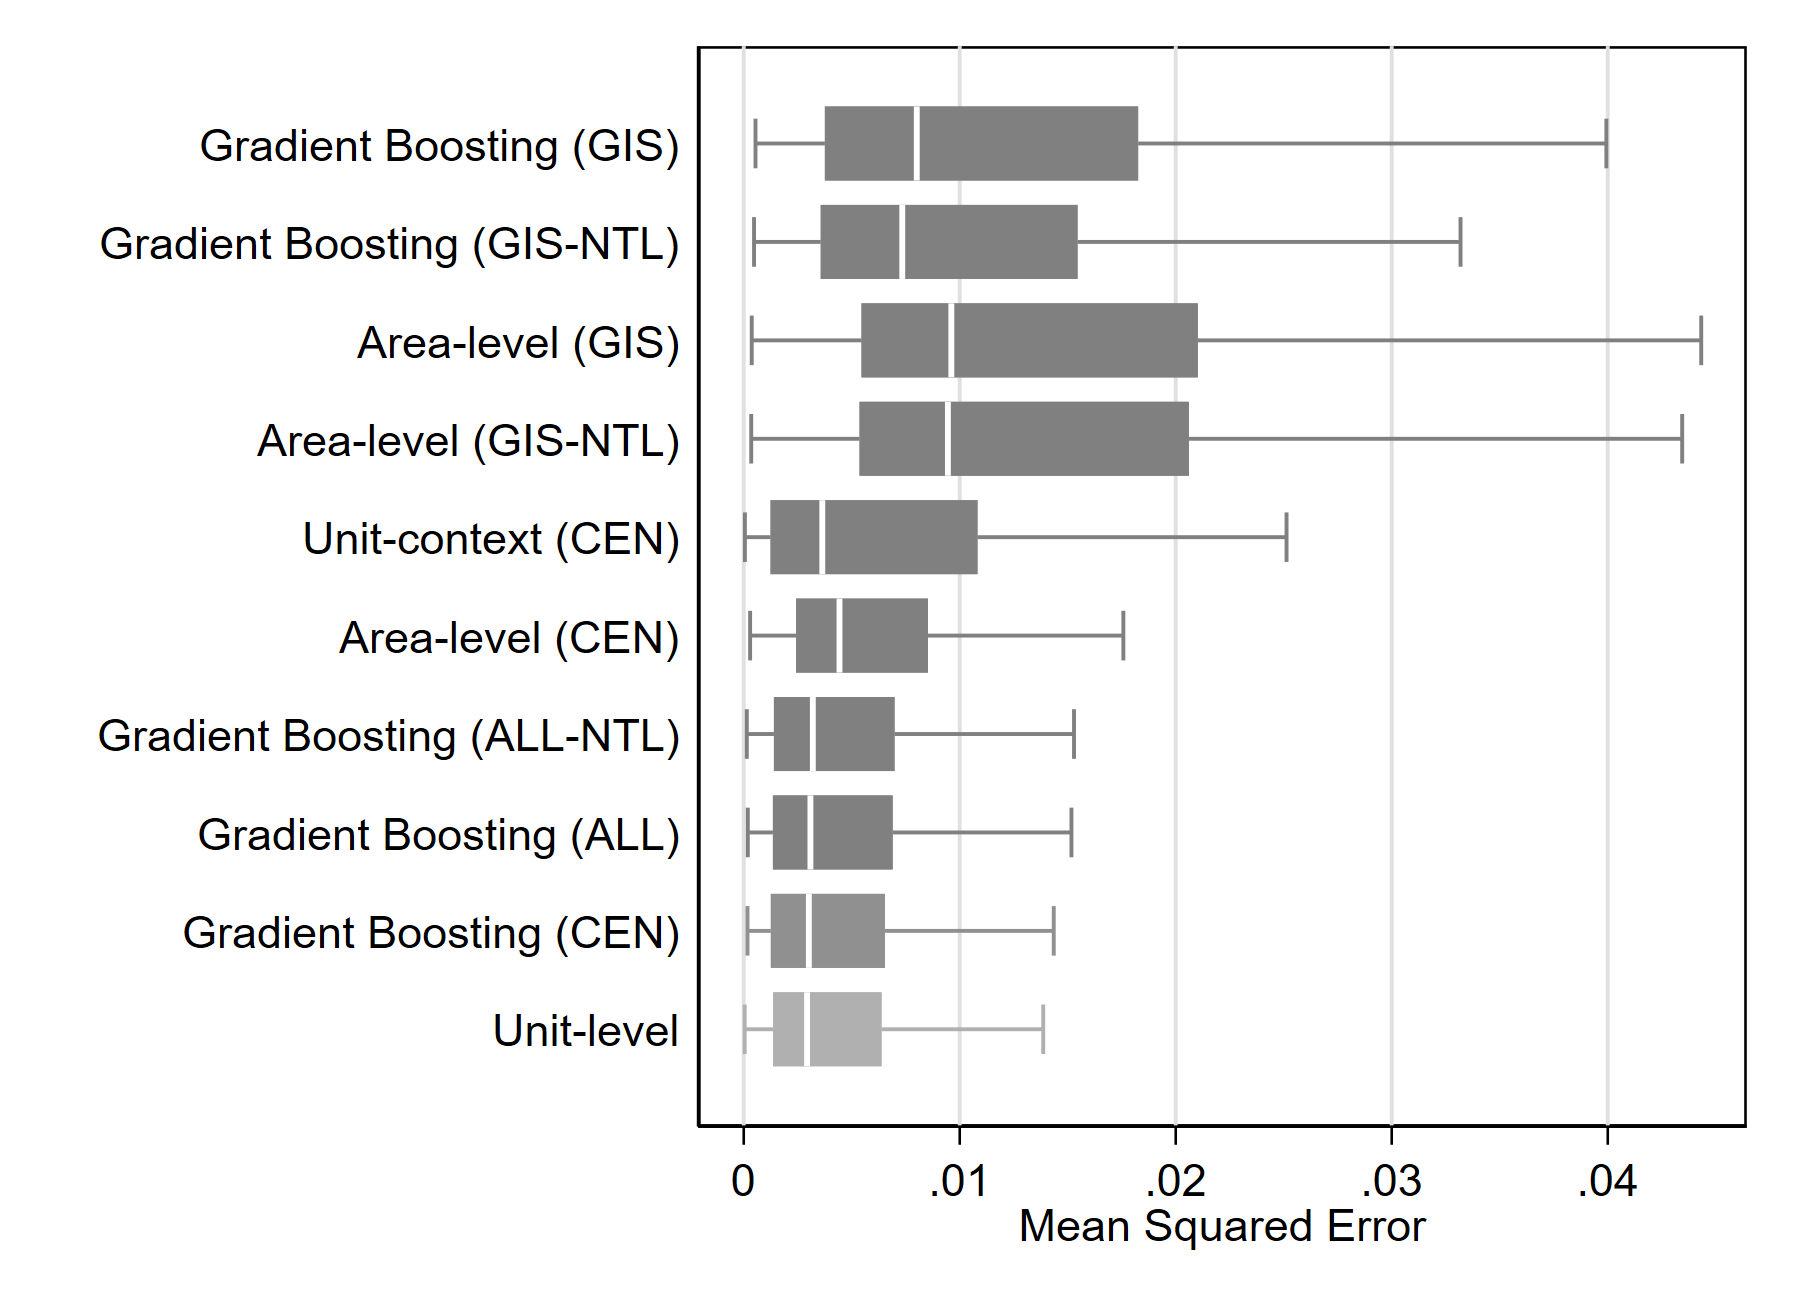
\includegraphics[scale=0.3]{Figure-2a}
\par\end{centering}
}\hspace{0cm}\subfloat[Targeting performance]{\begin{centering}
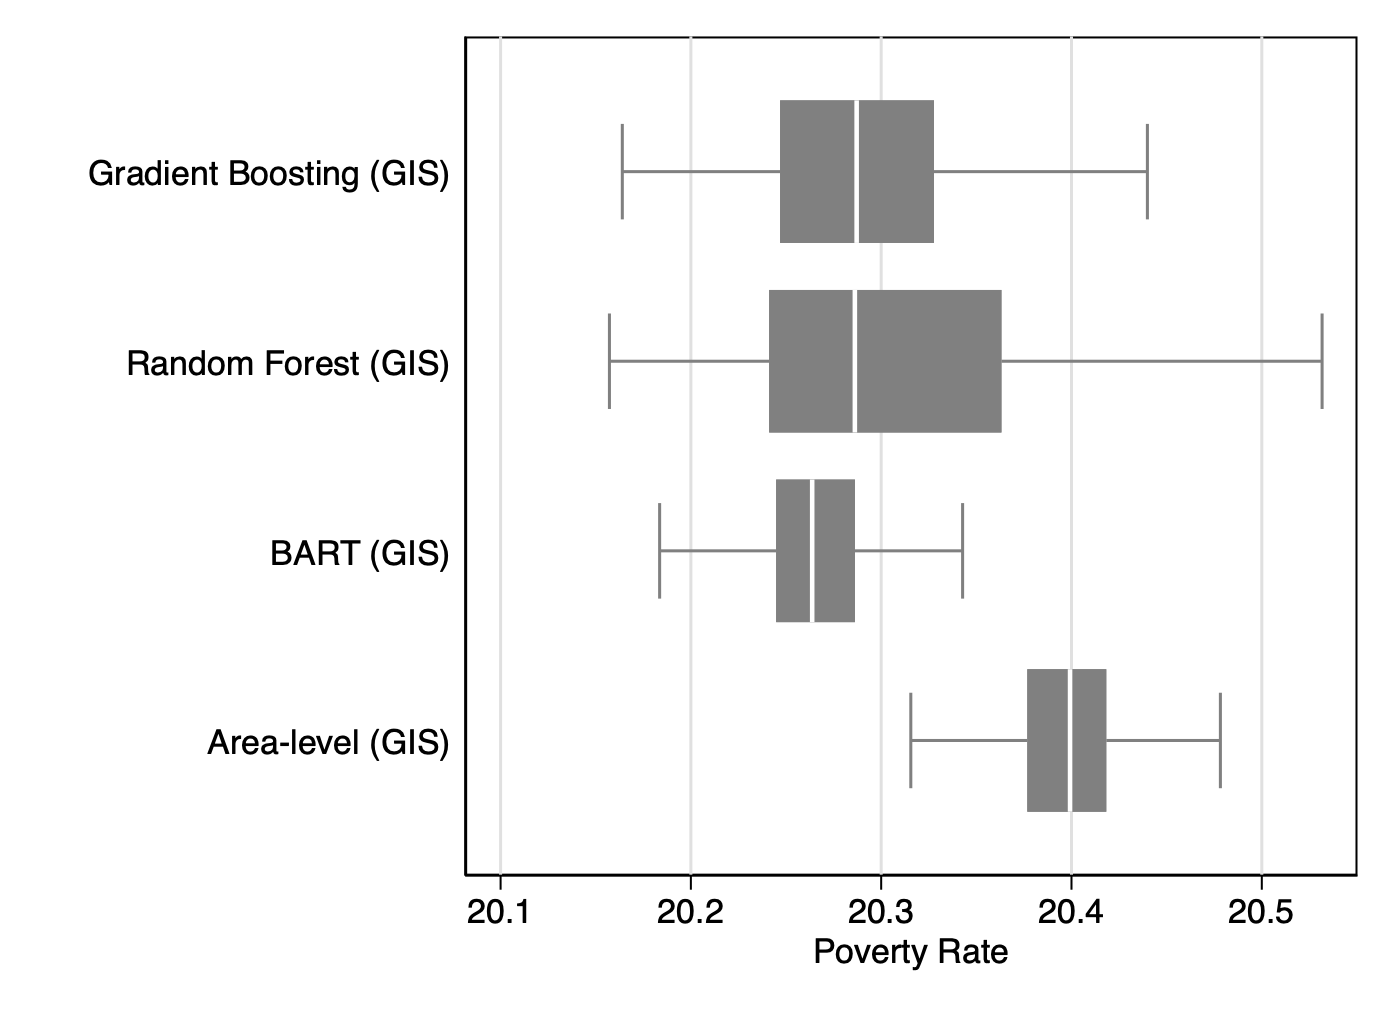
\includegraphics[scale=0.3]{Figure-2b}
\par\end{centering}
}
\par\end{centering}
\centering{}\caption{Mean squared error and targeting performance for alternative statistical
methods \protect\label{fig:alt_methods}}
\end{figure}

By contrast, Figure \ref{fig:alt_covariates} shows that implementing
gradient boosting with census-based covariates leads to notable performance
gains. The first two boxplots in panels (a) and (b) present the results
for gradient boosting with remotely-sensed and census-based covariates,
respectively. As a benchmark, we plot similar results for the area-level
model. Recall that when using remotely-sensed covariates, gradient
boosting achieves a median MSE of 0.007 and a median poverty rate
of 20.29. With census-based covariates, the median MSE falls to 0.003
and the median poverty rate falls to 20.02. Importantly, gradient
boosting with census-based covariates slightly outperforms the area-level
model, which achieves a median MSE of 0.004 and a median poverty rate
of 20.04 when using the same covariates. The under-performance of
the modern approach is thus largely driven by the remotely-sensed
covariates.

\begin{figure}
\begin{centering}
\subfloat[Mean squared error]{\begin{centering}
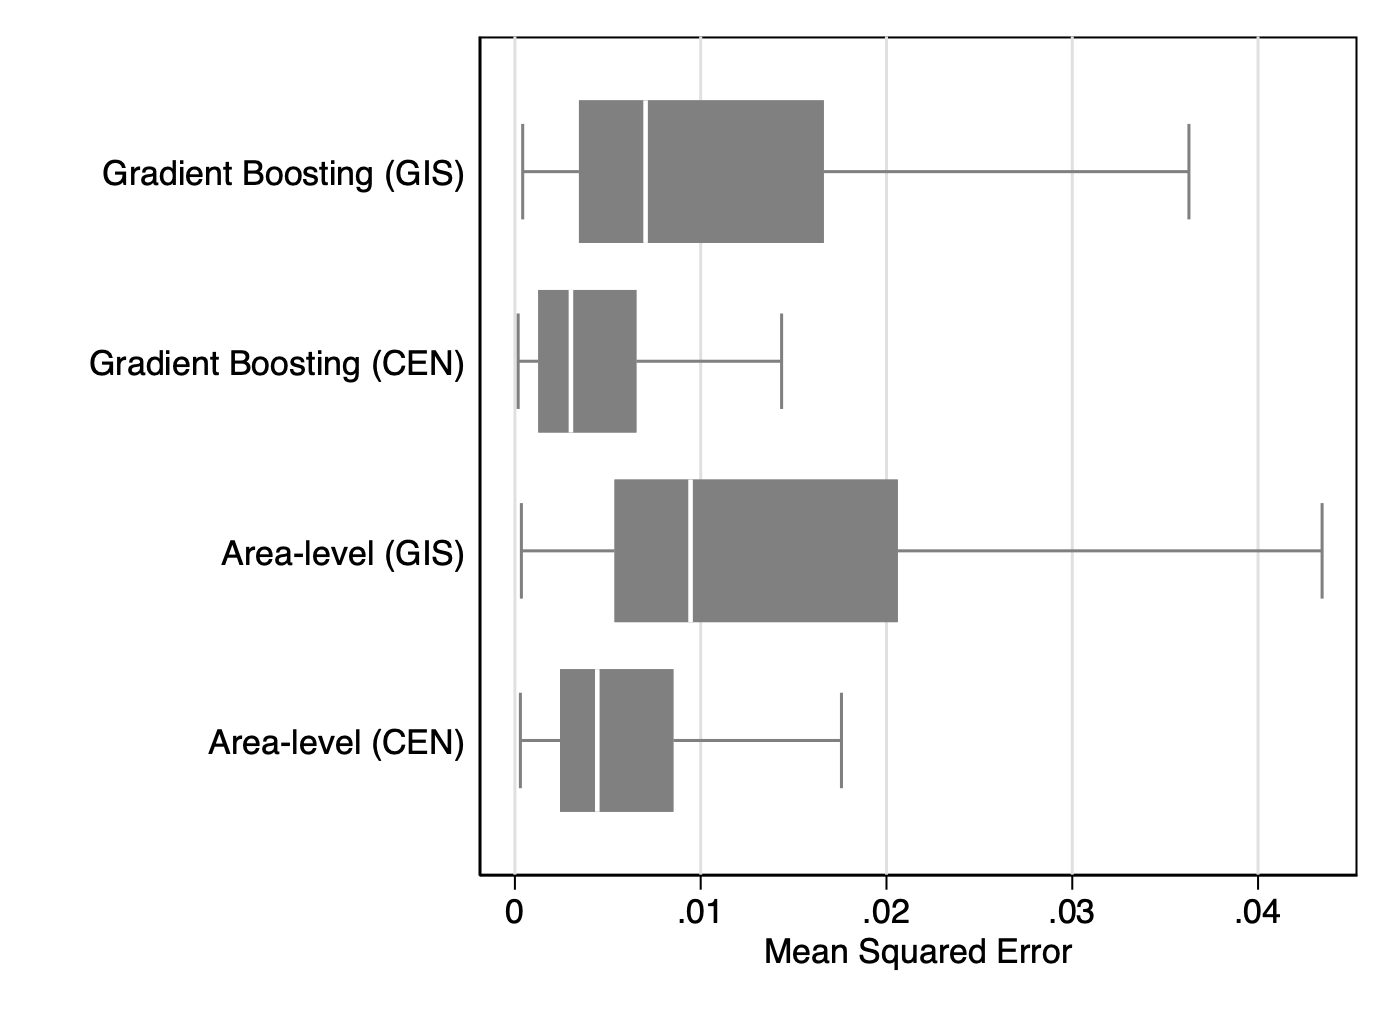
\includegraphics[scale=0.3]{Figure-3a}
\par\end{centering}
}\hspace{0cm}\subfloat[Targeting performance]{\begin{centering}
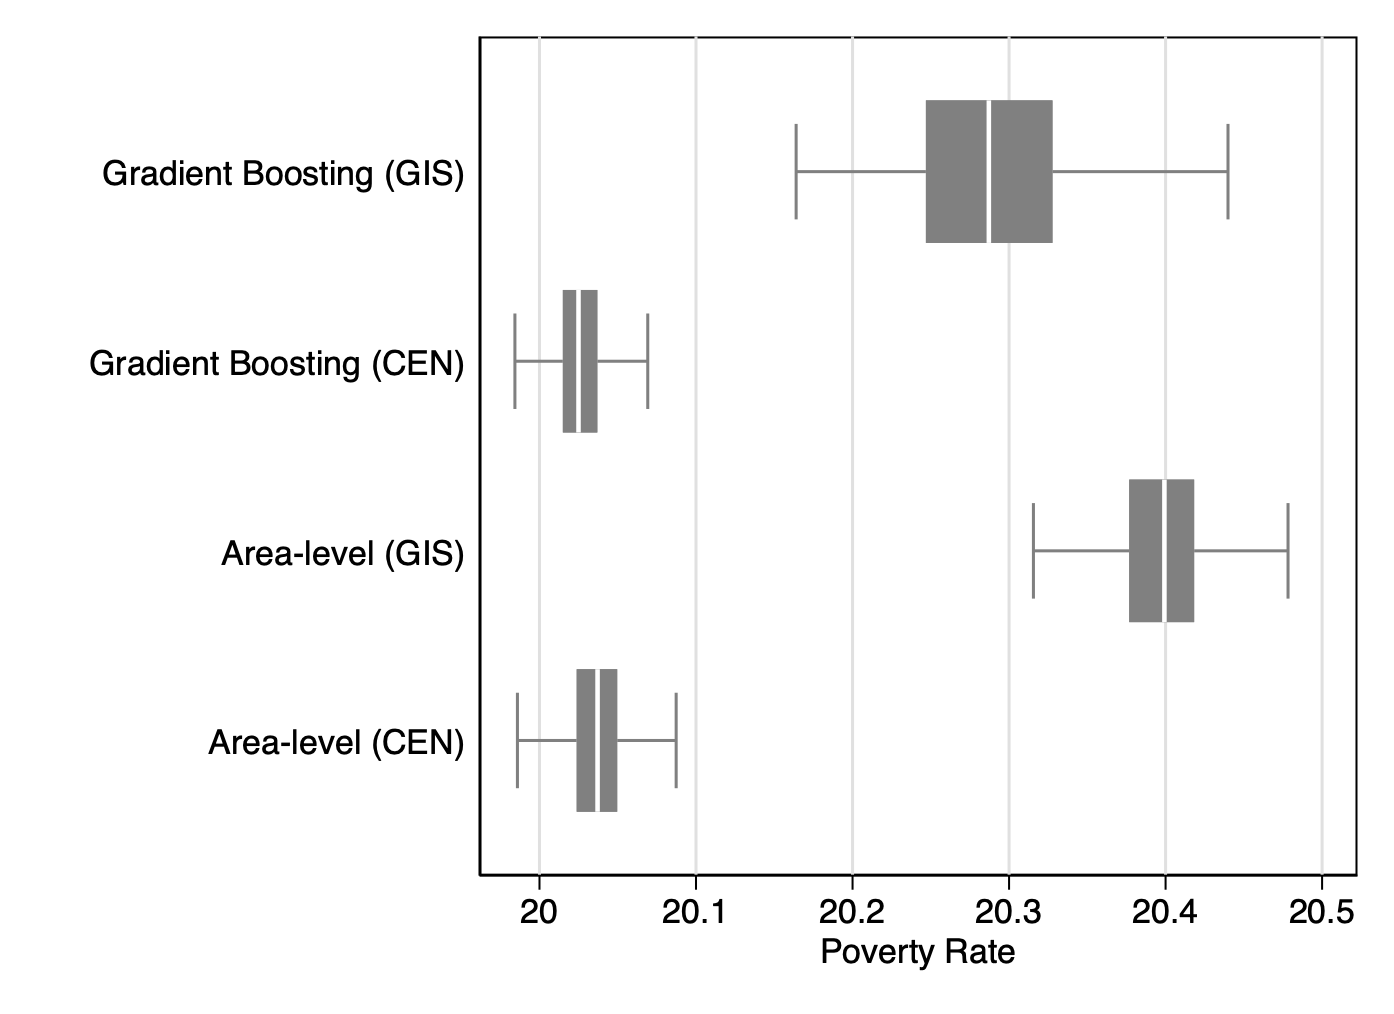
\includegraphics[scale=0.3]{Figure-3b}
\par\end{centering}
}
\par\end{centering}
\centering{}\caption{Mean squared error and targeting performance for alternative covariates
\protect\label{fig:alt_covariates}}
\end{figure}

Another way to see that the census-based covariates have greater predictive
capacity than the remotely-sensed covariates is by looking at feature
importance. One popular measure of feature importance summarizes the
gain (i.e., reduction of the loss function) associated with any given
feature. That is, for a given run of the model, feature importance
captures the average gain of a given feature, where the gains are
averaged across all trees in the model.\footnote{In addition, the average gains for a given run of the model are normalized
by dividing each by the sum of all average gains for that run.} Figure \ref{fig:feature} plots the 20 covariates with the highest
feature importance after running gradient boosting with both census-based
(``CEN'') and remotely-sensed (``GIS'') covariates on each sample
and averaging each covariate\textquoteright s importance across the
500 samples. We find that all of the top 10 covariates are census-based,
with only six remotely-sensed covariates entering the top 20. Note
also that the feature importances outside the top 10 are relatively
small in magnitude.

\begin{figure}
\begin{centering}
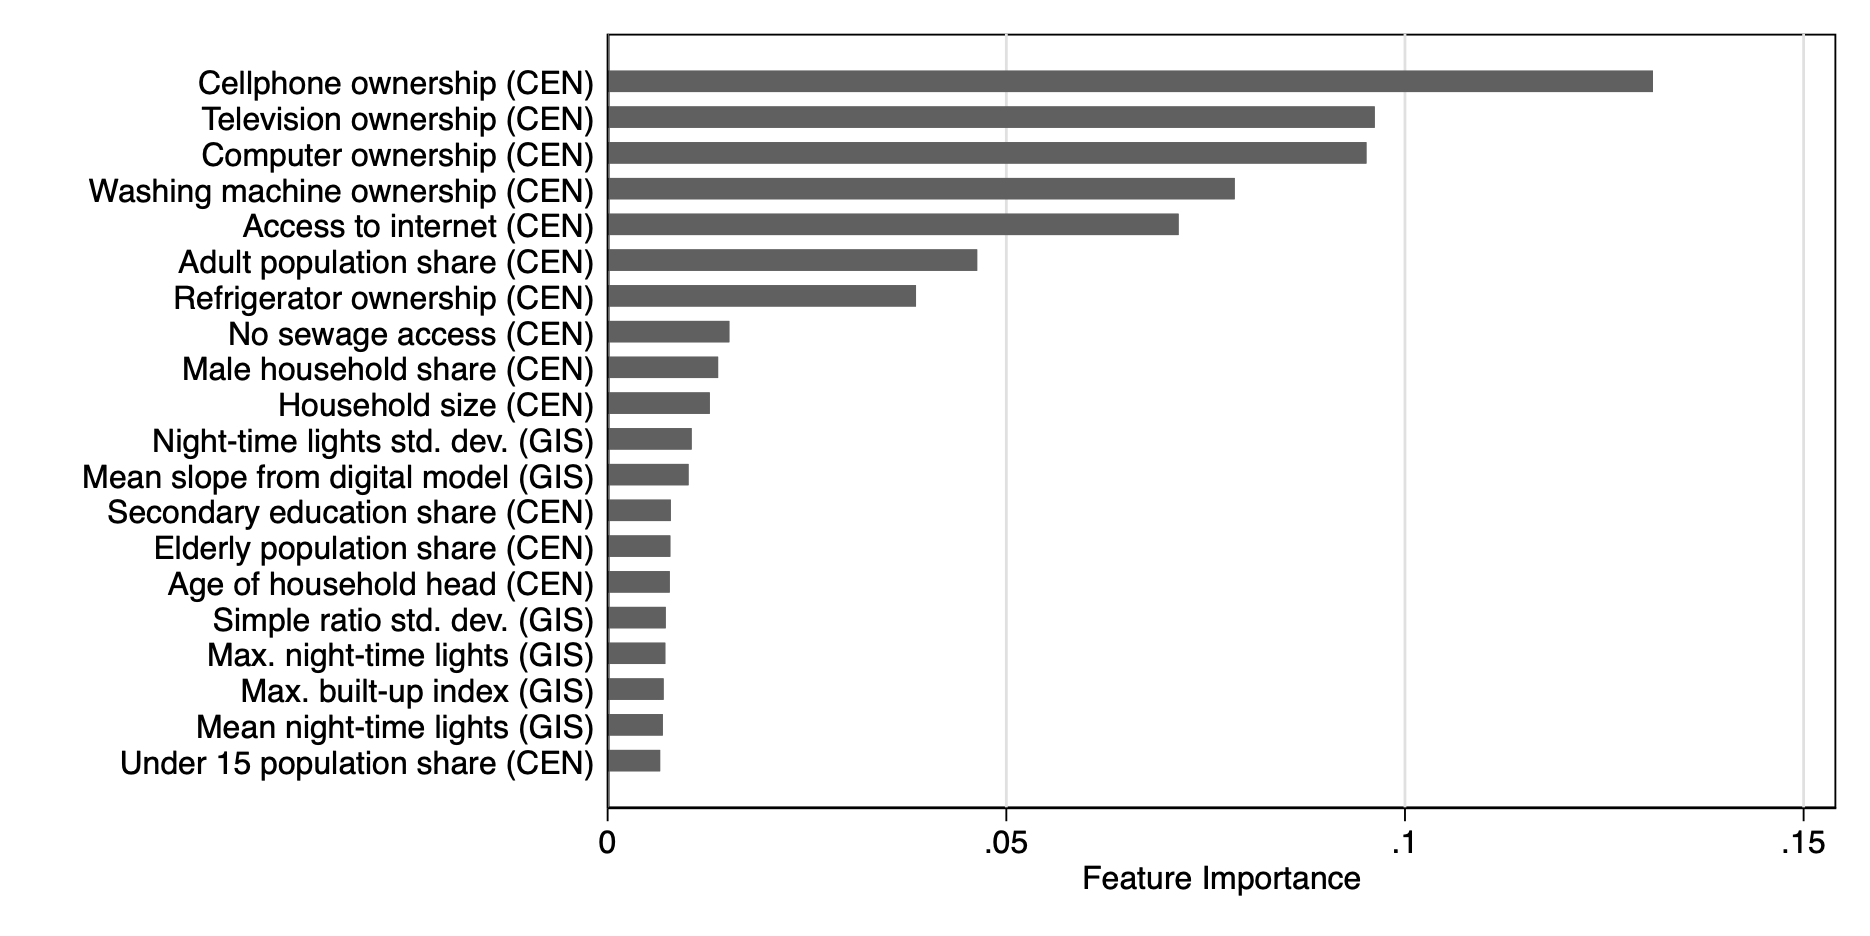
\includegraphics[scale=0.35]{Figure-4}
\par\end{centering}
\centering{}\caption{Feature importance\protect\label{fig:feature}}
\end{figure}

The above results suggest that gradient boosting can approximate the
performance of the unit-level model and outperform the area-level
model when using the same covariates. The aggregated nature of our
performance comparisons thus far, however, mask some important differences
between the methods. To illustrate these differences, we first use
the variance-bias decomposition presented in Eq. (\ref{eq:mseg})
and plot the two components independently. Panel (a) of Figure \ref{fig:decomposition}
presents boxplots summarizing the distribution of the variance component
across municipalities for select models. We see that gradient boosting
is associated with lower variance estimates than the area-level model
for any given set of covariates. For example, the median variance
for gradient boosting with remotely-sensed covariates is 0.002 whereas
the median variance for the area-level model with the same covariates
is 0.005. This variance reduction is an important advantage of gradient
boosting and the reason for its use of regularization.

\begin{figure}
\begin{centering}
\subfloat[Variance]{\begin{centering}
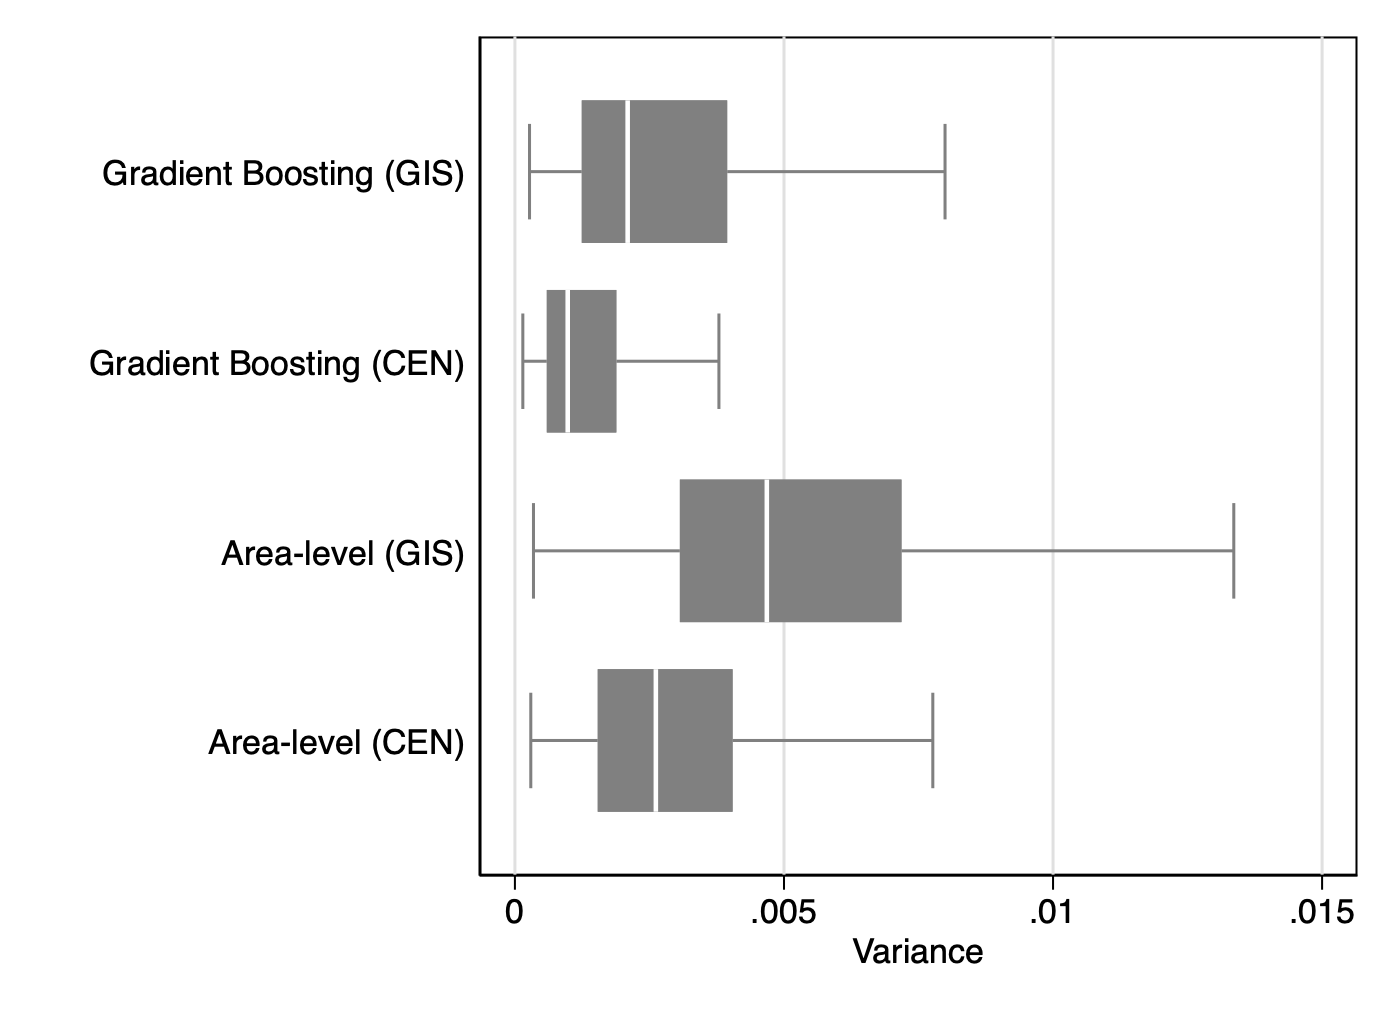
\includegraphics[scale=0.3]{Figure-5a}
\par\end{centering}
}\hspace{0cm}\subfloat[Bias]{\begin{centering}
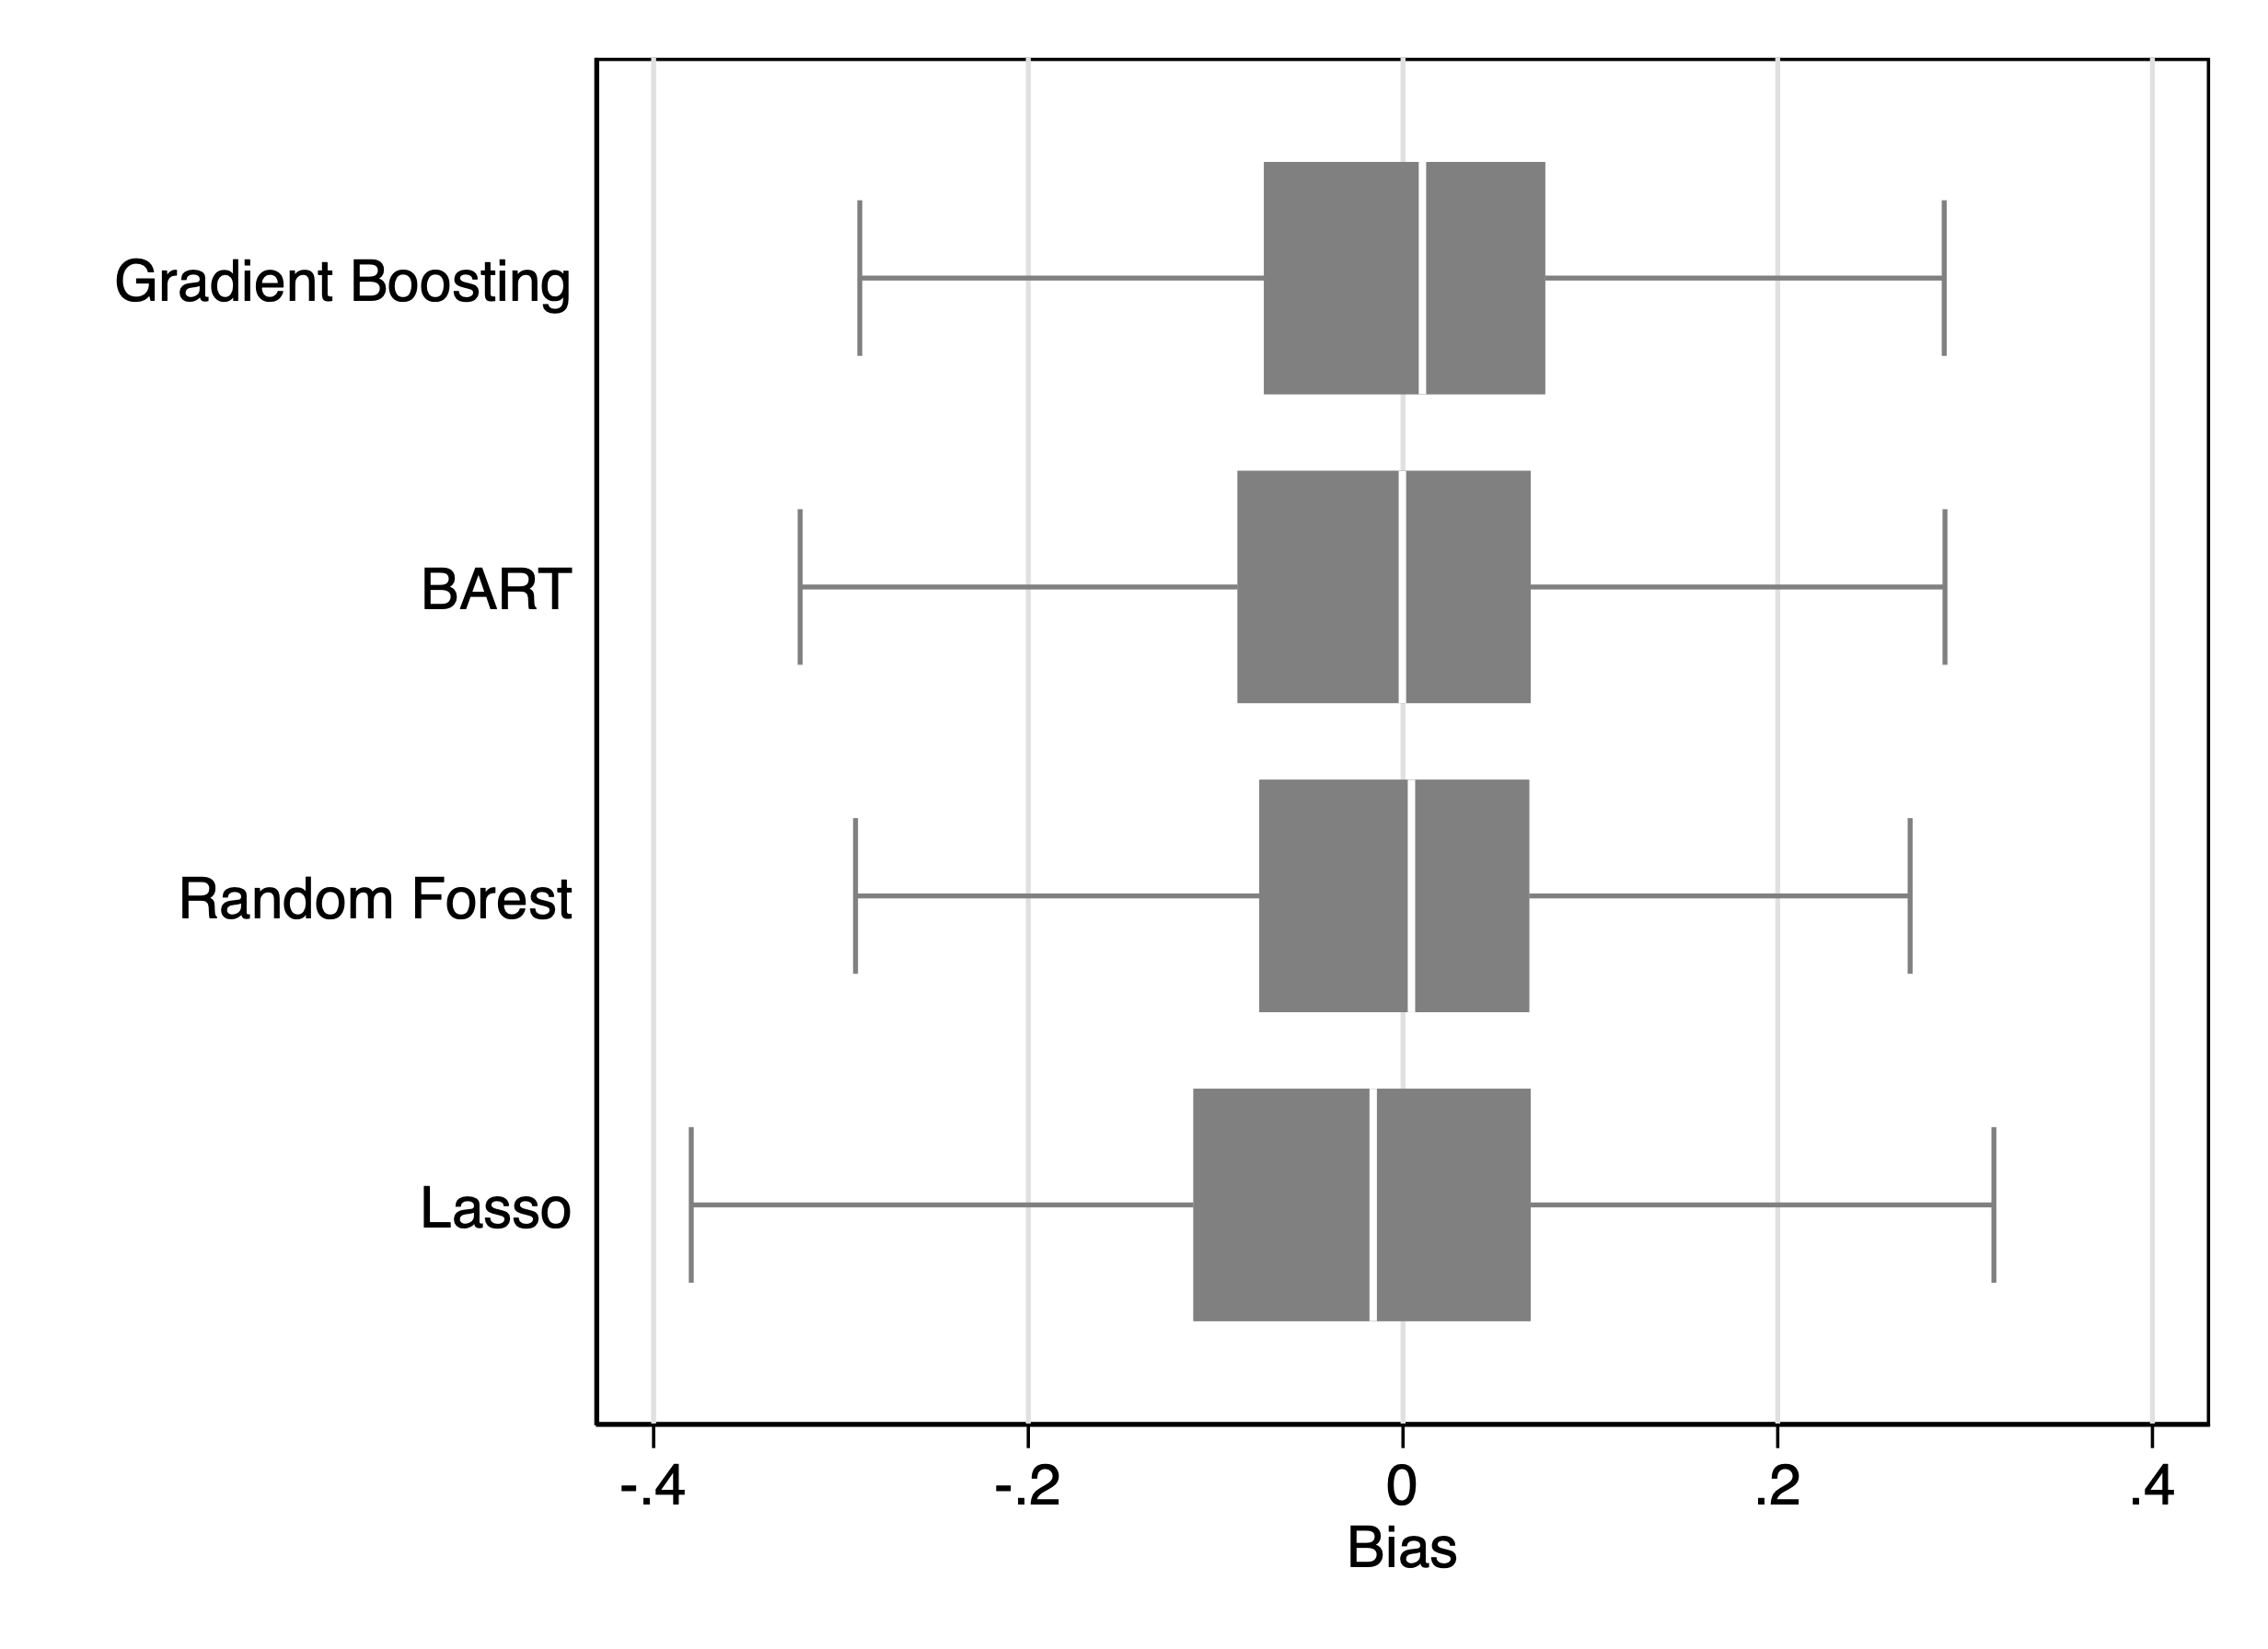
\includegraphics[scale=0.3]{Figure-5b}
\par\end{centering}
}
\par\end{centering}
\centering{}\caption{Variance-bias decomposition for select models \protect\label{fig:decomposition}}
\end{figure}

Panel (b) presents the bias component of the decomposition for the
same set of models and shows that all the models depicted are approximately
unbiased at the median.\footnote{The variance-bias decomposition shows that the MSE is the sum of the
variance and the squared bias of the estimates. To illustrate both
underestimates and overestimates, we do not square the bias estimates.} The models using remotely-sensed covariates nevertheless exhibit
wide variation in the bias estimates, implying that the estimated
poverty rates for some municipalities are severely biased. For example,
the minimum and maximum bias estimates for gradient boosting with
remotely-sensed covariates are -45 and 40 percentage points, respectively.
The area-level model exhibits similar variation in the bias estimates
when using remotely-sensed covariates, indicating that weak predictors
can produce considerable biases for both methods, at least for some
municipalities. While gradient boosting and the area-level model appear
to be similarly biased for any given covariate set, a closer look
at the source of these biases reveals an important shortcoming of
gradient boosting.

To this end, panel (a) of Figure \ref{fig:poverty_sampling} plots
the municipality-level bias estimates from select models on the true
municipality poverty rates. For each model, we fit a lowess curve
to the data to show the (weighted) average of the bias estimates at
different true poverty rates. The figure shows the source of the aforementioned
bias variability: both models with remotely-sensed covariates severely
overestimate poverty in the least poor municipalities and underestimate
poverty in the most poor municipalities. Stated differently, the models
with remotely-sensed covariates understate the spatial distribution
of poverty. This result occurs because the predictions collapse toward
the mean in the absence of informative covariates, which produces
predictable biases in the tails of the distribution. Interestingly,
for both covariate types, the area-level model is less biased for
the poorest municipalities.

\begin{figure}
\begin{centering}
\subfloat[Bias by poverty rate]{\begin{centering}
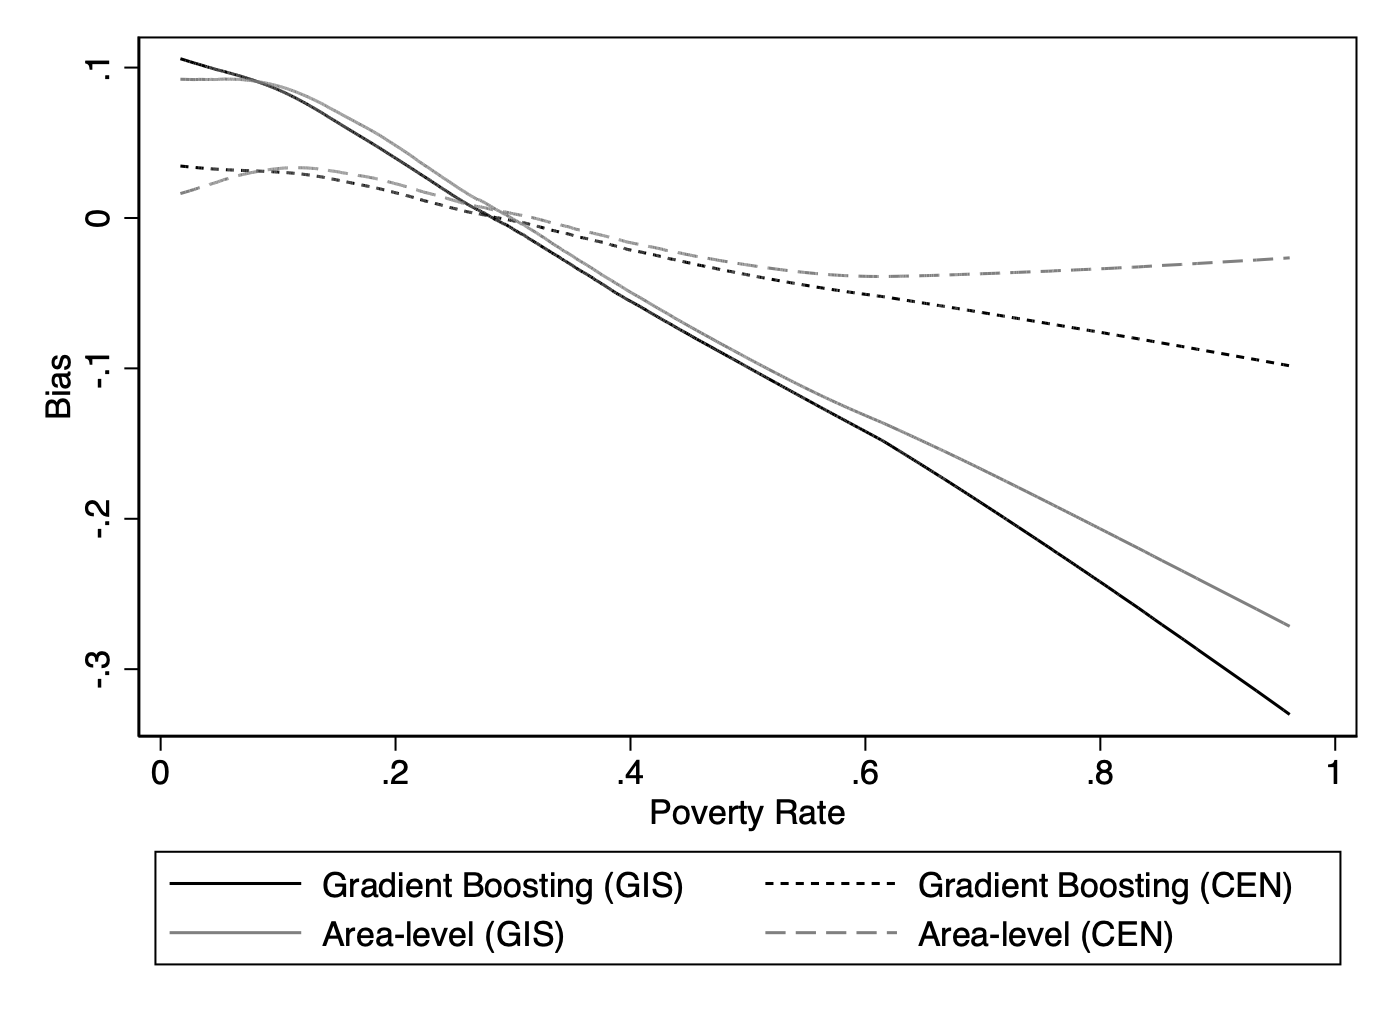
\includegraphics[scale=0.3]{Figure-6a}
\par\end{centering}
}\hspace{0cm}\subfloat[Bias by sampling frequency]{\begin{centering}
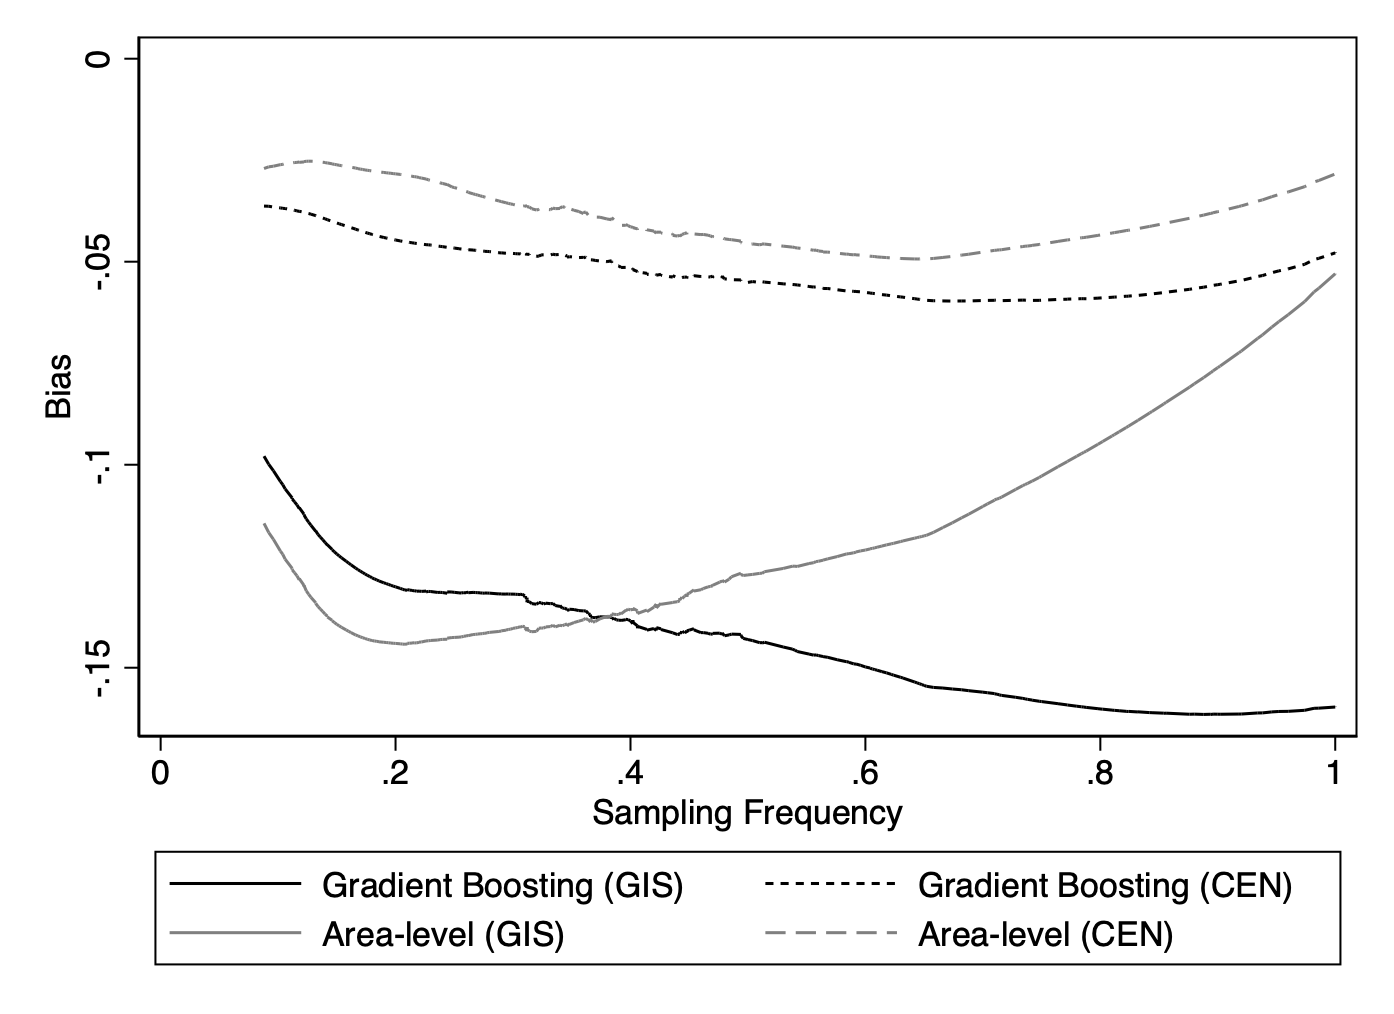
\includegraphics[scale=0.3]{Figure-6b}
\par\end{centering}
}
\par\end{centering}
\centering{}\caption{Bias by poverty rate and sampling frequency\protect\label{fig:poverty_sampling}}
\end{figure}

Panel (b) in Figure \ref{fig:poverty_sampling} shows that an important
reason for the area-level model's reduced bias is that its in-sample
predictions are a weighted average of the model-based estimates and
the (unbiased) direct estimates.\footnote{See Section \ref{sec:methods} for details. By contrast, gradient
boosting relies exclusively on the model-based estimates and only
incorporates the direct estimates when fitting the model.} For each model depicted, we focus on the 20 percent of municipalities
with the lowest true poverty rate, plot the municipality-level bias
estimates on the frequency with which a municipality was sampled,
and then fit a lowess curve to the data. The sampling frequencies
capture the proportion of samples for which a municipality received
an in-sample prediction, thus benefitting from the area-level model's
averaging procedure. As expected, we see that the area-level model
is less biased for municipalities with higher sampling frequencies.
The performance disparity is especially pronounced among the models
with remotely-sensed covariates, as the area-level model is roughly
10 percentage points less biased at the highest sampling frequencies.

These latter results highlight an important methodological difference
between the modern and traditional approaches. In particular, the
machine-learning methods used for poverty mapping were developed for
out-of-sample prediction and ignore the direct estimates after fitting
the model. The traditional methods, by contrast, were developed specifically
for poverty mapping and recognize that mapping is partly an in-sample
prediction problem. The traditional methods thus use the direct estimates
after fitting the model and weight them more heavily when the covariates
are less informative. Interestingly, this highlights another concern
with using direct estimates to assess model performance: traditional
methods are designed to be less predictive of direct estimates when
the model is more informative. The main point here is nevertheless
that our results are in line with the expectation that traditional
methods will exhibit less in-sample bias, particularly in the presence
of weak covariates.

\section{Conclusion\protect\label{sec:conclusion}}

Machine-learning approaches to poverty mapping have become increasingly
popular in recent years. In contrast to traditional mapping procedures,
modern machine-learning methods rely on non-parametric statistical
techniques applied to remotely-sensed data, such as satellite imagery
or call detail records. In addition, machine-learning approaches routinely
conduct model assessment using the $R^{2}$, which is often calculated
by regressing direct, survey-based poverty estimates on model predictions.
While direct estimates are unbiased, they can be imprecise measures
of true poverty rates and, as a result, it is unclear whether this
approach to assessment is informative of model performance. In this
paper, we thus conducted a more rigorous assessment of the machine-learning
approach to poverty mapping by using the Mexican Intercensal Survey
for several design-based simulation experiments.

To motivate our experiments, we outlined several ways that the $R^{2}$
can be a misleading measure of model performance: it is biased downward
when direct estimates are used as the reference measure of model performance,
it is insensitive to differences in location and scale between the
reference measure and the model predictions, and it is normalized
by the variance of the reference measure. The limitations of the standard
validation procedure are due both to the $R^{2}$ metric itself and
from applying the $R^{2}$ to direct poverty estimates rather than
true poverty measures. Our experiments address these limitations in
two ways: (1) we assess model performance using data that allows us
to use true poverty indicators as the reference measures, and (2)
we emphasize validation metrics that are sensitive to systematic biases
in the poverty estimates and avoid the normalization issue.

Our results showed that the modern approach to poverty mapping under-performs
relative to the traditional approach both in terms of mean squared
error and poverty reduction. We found that this under-performance
is driven by the modern approach's reliance on remotely-sensed covariates.
When using the same covariates, we found that machine learning performs
comparably to the unit-level model and slightly outperforms the area-level
model. We then showed that the performance advantage of machine learning
relative to the area-level model is due to its variance-reduction
properties, namely its use of regularization. The cost of such variance
reduction, however, is that machine learning exhibits more bias in
the tails of the poverty distribution than the area-level model. This
bias-variance tradeoff is especially stark in the context of remotely-sensed
covariates, which suggests that the quality of the available data
is an important consideration when choosing between parametric and
non-parametric mapping methods.

Our analysis has several practical implications for poverty mapping.
For one, producers and users of poverty maps should exercise caution
when using $R^{2}$ as a model assessment tool, especially when it
is calculated using direct poverty estimates as the reference measure.
Poverty maps should ideally be validated using a ground truth and
alternative validation metrics, such as the mean squared error and
targeting performance.\footnote{See \citet{tzavidis2018start} for additional discussion.}
The data requirements for constructing a credible ground truth are
nevertheless demanding and unlikely to be met in many country contexts.
One possible strategy for researchers in these cases is to use richer
data from other countries to assess their methodological decisions,
particularly decisions that have not been previously validated. The
Mexican Intercensal Survey, for example, is publicly available on
the INEGI website.\footnote{See https://en.www.inegi.org.mx/programas/intercensal/2015. For the
remotely-sensed data in the same year, see https://www.inegi.org.mx/investigacion/geomediana.
The processed data for our simulation experiments are also available
upon request. } 

Our results also highlight that covariate quality has important implications
for the practice of poverty mapping. Most obviously, the limited predictive
capacity of remotely-sensed covariates suggests that researchers should
incorporate census-based covariates whenever possible. Perhaps more
interestingly, our results suggest that the quality of the available
covariates has implications for the choice of statistical model, particularly
in off-census years. With high-quality covariates, there are only
minor performance differences between the non-parametric and parametric
approaches to estimating poverty maps. Machine learning is a reasonable
choice in this case, as it performs slightly better overall with only
minimal increases in bias. With lower-quality covariates, however,
the modest overall advantage of machine learning is coupled with substantial
increases in bias for some areas. Machine learning should be used
with caution in this case, especially when poverty maps are needed
to understand absolute poverty levels.

We have identified several limitations of the modern approach to poverty
mapping, but our analysis has its own drawbacks. We have focused on
measuring income poverty and have not considered the performance of
the modern approach when used in the context of other welfare measures
(e.g., wealth).\footnote{In particular, see \citet{hall2023review} for detailed discussion
on the capacity of remotely-sensed data to predict alternative welfare
measures.} We have also only examined the modern approach using the Mexican
Intercensal Survey and remotely-sensed data available at the same
time. Other types of passively-collected data (e.g., call detail records)
or experiments using data from other countries could produce different
results. Finally, there are other possible applications of machine
learning to poverty mapping that we have not considered, such as extracting
numerical covariates from high-dimensional data sources. Each of these
limitations suggests a potential area for future research. 

An additional area for future research would be to develop strategies
to correct the $R^{2}$ for its various limitations. For example,
one might correct for measurement error in the direct estimates by
multiplying the estimated $R^{2}$ by the reciprocal of the bias term.
This strategy would require estimating the variance of the measurement
error associated with the direct estimates. Relatedly, note that our
derivation of this bias relies on the assumption of classical measurement
error, which may be violated in practice (e.g., if poorer or richer
households are less likely to be sampled). Another topic for future
research would then be to derive the bias under less stringent assumptions.
Finally, as measurement error in the direct estimates is not the only
concern with $R^{2}$, future research could consider applying multiple
adjustments simultaneously. 

\pagebreak{}

\bibliographystyle{apalike}
\bibliography{References}

\end{document}
